\documentclass[12pt]{article}
\usepackage{background}
\usepackage{graphicx}
\usepackage[margin=1in]{geometry}
\usepackage{setspace}
\usepackage{hyperref}
\usepackage{xcolor}
\usepackage{tikz}
\usepackage{listings}
\usepackage{xcolor}
\usepackage{float}
\usepackage{subcaption}
\lstset{
  language=Python,
  backgroundcolor=\color{black!5},   % light gray background
  basicstyle=\ttfamily\small,         % Monospaced font for code
  breaklines=true,                    % Line wrapping
  keywordstyle=\color{blue},           % Keywords in blue
  commentstyle=\color{green},         % Comments in green
  stringstyle=\color{red},            % Strings in red
  identifierstyle=\color{black},      % Identifiers in black
  morekeywords={def,class}, 
           % Function and class names in bold
  morekeywords={import, as},      % Add extra keywords to be highlighted
                      % Space between line numbers and code
  frame=single,                       % Single line frame around the code
  rulecolor=\color{black},            % Frame color
  tabsize=4,                          % Number of spaces per tab
  showstringspaces=false              % Don't underline spaces in strings
}
\backgroundsetup{
  scale=0.5,                       % Scale the image
  color=black,                   % Image color (you can change it)
  opacity=0.1,                     % Opacity (1 for full opacity)
  angle=0,                       % Image rotation
  position=current page.center,   % Position at the center of the page
  vshift=-5cm,                    % Vertical shift
  hshift=0cm,                    % Horizontal shift
  contents={
\includegraphics[width=\paperwidth, height=\paperheight]{figs/logo.jpg}}  % Include the image
}

\usepackage{amsmath}

\begin{document}

\begin{titlepage}
    \centering
    {\Huge \bfseries  Lissajous Figures and Capturing One-Time Events on a CRO

 \par}
    \vspace{1cm}
    
\includegraphics[width=5cm]{figs/logo.jpg} % Replace with your logo file
    \vspace{1cm}
   
    {\Large \bfseries Lab Assignment : 01 \par}
    \vspace{0.5cm}
   
    {\large EE1200: Electrical Circuits Lab \par}
    \vspace{2cm}
   
\begin{tabular}{ll}
    \textbf{S. Rohith Sai} & \textbf{EE24BTECH11061} \\
    \textbf{Y. Harsha Vardhan Reddy} & \textbf{EE24BTECH11063} \\
\end{tabular}
\vspace{1cm}

\end{titlepage}
\newpage
\tableofcontents
\newpage
\section{Overview of the Project}

The primary objective of this experiment is to study and observe the behavior of Lissajous figures, as well as to explore the process of capturing a single event using an oscilloscope and a function generator. These techniques are fundamental in electrical engineering for analyzing waveforms and signals, and they serve as the basis for many types of signal processing and measurement tasks.

\subsection{Objective}
The objective of this experiment is to:
\begin{itemize}
    \item Generate and observe Lissajous figures using different frequencies and phase relationships.
    \item Understand the principles of triggering and signal acquisition by capturing a single event.
    \item Gain hands-on experience with the oscilloscope and function generator as measurement tools.
\end{itemize}

\subsection{Equipment Used}

The following equipment was used in this experiment:

\begin{itemize}
    \item \textbf{Oscilloscope (Agilent Technologies DSO3062A)}: The Agilent Technologies DSO3062A is a digital storage oscilloscope with a 60 MHz bandwidth and a sample rate of up to 1 GSa/s. It was used to visualize and analyze the waveforms generated by the function generator. 
    
    \item \textbf{Function Generator (Tektronix AFG1022)}: The Tektronix AFG1022 is a signal generator capable of producing sine, square, and other types of waveforms. It was used to generate the input signals for the experiment. 
    
    \item \textbf{Probes}: Two passive probes were used to connect the oscilloscope to the circuit and to measure the signal outputs from the function generator. These probes allowed for precise signal monitoring and waveform observation.
\end{itemize}

\section{\textbf{Introduction to oscilloscope}}
An oscilloscope is an electronic test instrument that graphically displays varying signal voltages, making it essential for diagnosing and analyzing electronic circuits
\subsection{ Purpose}
An oscilloscope is used to:
\begin{itemize}
    \item Visualize electrical signals in real time.
    \item Measure signal parameters like amplitude, frequency, time period, and phase.
    \item Troubleshoot and debug electronic circuits.
\end{itemize}

\subsection{ Key Components}
\begin{itemize}
    \item \textbf{Display Screen:} Shows the graphical representation of the signal (usually as a waveform).
    \item \textbf{Vertical (Y-axis):} Represents the voltage (amplitude of the signal).
    \item \textbf{Horizontal (X-axis):} Represents time.
    \item \textbf{Probes:} Connect the oscilloscope to the circuit under test.
    \item \textbf{Control Panels:}
    \begin{itemize}
        \item \textbf{Vertical Controls:} Adjust the amplitude scale.
        \item \textbf{Horizontal Controls:} Adjust the time scale.
        \item \textbf{Trigger Controls:} Stabilize the waveform for repetitive signals.
    \end{itemize}
\end{itemize}
\subsection{Key Terms}
\begin{itemize}
    \item \textbf{Time Base (Horizontal Scale):} The time per division on the X-axis (e.g., 1 ms/div).
    \item \textbf{Voltage Scale (Vertical Scale):} The voltage per division on the Y-axis (e.g., 1 V/div).
    \item \textbf{Triggering:} Synchronizes the waveform display for stability.
\end{itemize}

\subsection{Basic Operation}
\begin{enumerate}
    \item \textbf{Connect the Probe:} Attach the probe to the signal source.
    \item \textbf{Set Vertical Scale:} Adjust the volts/division to match the signal amplitude.
    \item \textbf{Set Horizontal Scale:} Adjust the time/division for the desired time resolution.
    \begin{itemize}
        \item The \textbf{Auto-Scale} button on an oscilloscope is a convenient feature that automatically adjusts the display settings, such as the time base, vertical scale, and trigger level, to optimally fit the signal within the screen. This allows users to quickly visualize the waveform without the need for manual adjustments, making it particularly useful for identifying unknown signals or performing quick diagnostics.
    \end{itemize}
    \item \textbf{Trigger the Signal:} Adjust the trigger settings to stabilize the waveform.
    \begin{itemize}
        \item The trigger in an oscilloscope is a control mechanism that stabilizes a repeating signal for display. It determines when the oscilloscope begins capturing data by defining a specific condition, such as a voltage level or edge direction (rising or falling).
        

    \end{itemize}
    \item \textbf{Observe the Waveform:} Analyze the amplitude, frequency, and shape.
\end{enumerate}

\subsection{Applications}
\begin{itemize}
    \item Testing signal integrity.
    \item Debugging circuits.
    \item Measuring parameters like rise time, duty cycle, and phase difference.
    \item Observing noise or interference in signals.
\end{itemize}
\section{Difference Between 1x and 10x Oscilloscope Probe Settings}

The \textbf{1x} and \textbf{10x} settings on an oscilloscope probe determine the attenuation factor, affecting signal measurement and display. Below is a summary of the key differences:

\begin{itemize}
    \item \textbf{1x Setting (No Attenuation):}
    \begin{itemize}
        \item Passes the input signal directly (1:1 ratio).
        \item Lower bandwidth, typically a few MHz.
        \item Lower input impedance (\(1~\mathrm{M\Omega}\) in parallel with higher capacitance, e.g., \(100~\mathrm{pF}\)).
        \item Causes more circuit loading, distorting signals.
        \item Suitable for low-frequency, low-impedance signals.
    \end{itemize}

    \item \textbf{10x Setting (10:1 Attenuation):}
    \begin{itemize}
        \item Attenuates the input signal by a factor of 10.
        \item Higher bandwidth, typically tens to hundreds of MHz.
        \item Higher input impedance (\(10~\mathrm{M\Omega}\) in parallel with lower capacitance, e.g., \(10~\mathrm{pF}\)).
        \item Minimizes circuit loading, maintaining signal integrity.
        \item Ideal for high-frequency or sensitive circuits.
    \end{itemize}
\end{itemize}

\begin{table}[H]
\centering
\renewcommand{\arraystretch}{1.5}
\setlength{\tabcolsep}{10pt}
\caption{Comparison of 1x and 10x Probe Settings}
\begin{tabular}{@{}|p{4cm}|p{5cm}|p{5cm}|@{}}
\hline
\textbf{Feature}          & \textbf{1x Setting}                             & \textbf{10x Setting}                            \\ \hline
\textbf{Attenuation}      & 1:1 (No attenuation)                           & 10:1 (Signal reduced by 10x)                   \\ \hline
\textbf{Bandwidth}        & Low (e.g., a few MHz)                          & High (Tens to hundreds of MHz)                 \\ \hline
\textbf{Input Impedance}  & \(1~\mathrm{M\Omega} \text{(or)} 100~\mathrm{pF}\) & \(10~\mathrm{M\Omega} \text{(or)} 10~\mathrm{pF}\) \\ \hline
\textbf{Signal Loading}   & High (More distortion)                         & Low (Better signal integrity)                  \\ \hline
\textbf{Use Case}         & Low-frequency, low-impedance signals           & High-frequency, sensitive circuits             \\ \hline
\end{tabular}
\end{table}
\section{Precautions while setting up an oscilloscope}
\begin{itemize}
    \item \textbf{Proper Grounding:} Ensure the oscilloscope and probes are properly grounded to avoid ground loops or electrical hazards.
    \item \textbf{Correct Probe Setting:} Match the probe attenuation (1x or 10x) with the oscilloscope's settings.
    \item \textbf{Input Range:} Set the vertical scale to avoid overloading the input and potential damage.
    \item \textbf{Trigger Settings:} Adjust the trigger level and mode for a stable display of the waveform.
    \item \textbf{Environmental factors: } Minimize interference by keeping the oscilloscope away from strong electromagnetic fields. 
    \item \textbf{Coupling modes: }\\
\begin{tabular}{@{}|p{4cm}|p{5cm}|p{5cm}|@{}}
\hline
\textbf{Feature}          & \textbf{DC Coupling}                       & \textbf{AC Coupling}                       \\ \hline
\textbf{Signal Components} & Displays both DC and AC components        & Displays only AC components (DC blocked)   \\ \hline
\textbf{Baseline}          & Shows the true signal baseline            & Centers the AC signal at 0 V              \\ \hline
\textbf{Use Case}          & Analyzing signals with DC offset          & Focusing on small AC variations           \\ \hline
\end{tabular}\\
\textbf{Selection tip:}\\
\begin{itemize}
    \item Use \textbf{DC-coupling} when you need to see the full signal, including any offset or steady-state voltage.
    \item Use \textbf{AC-coupling} when you're interested only in the varying (AC) part of the signal.
\end{itemize}
\end{itemize}
\section{Introduction to Function Generator}

A \textbf{function generator} is an electronic test instrument used to produce various waveforms, such as sine, square, triangle, and pulse waves, at different frequencies and amplitudes. It is commonly used in laboratories to test circuits, components, and systems by providing a known input signal for measurement or simulation. 

Key features include:
\begin{itemize}
    \item Adjustable frequency, amplitude, and offset.
    \item Output waveforms: sine, square, triangle, pulse, and others.
    \item Can generate both low and high-frequency signals, typically from a few Hz to several MHz.
    \item Used for testing frequency response, signal processing, and circuit analysis.
\end{itemize}
\section{Precautions While Setting Up a Function Generator}

\begin{itemize}
    \item \textbf{Check Output Settings:} Ensure the output waveform type, frequency, and amplitude are set correctly to avoid damage to connected circuits.
    \item \textbf{Limit Signal Amplitude:} Verify the output voltage is within the safe range for the device under test (DUT) to prevent overloading or damage.
    \item \textbf{Use align-phase:} At regular intervals use align-phase button/option to ensure that the phase is appropriately set according to the input values because there might be small error in the phase (especially, when working with trigonometric functions like sine wave).
\end{itemize}
\section{Producing Lissajous Figures(Task-1)}
\subsection{Working of an Cathode Ray Oscilloscope(CRO): }
A Cathode Ray Oscilloscope (CRO) is used to visualize electrical signals in the form of waveforms. It consists of the following main components:

\begin{itemize}
    \item \textbf{Electron Gun:} Emits an electron beam directed towards the screen.
    \item \textbf{Vacuum Tube:} Contains the electron gun and the phosphor-coated screen.
    \item \textbf{Deflection Plates:} Horizontal (X-axis) and vertical (Y-axis) plates control the movement of the electron beam.
    \item \textbf{Phosphor-Coated Screen:} Glows when struck by the electron beam, forming the visible waveform.
    \item \textbf{Time Base:} Controls the horizontal sweep of the electron beam, representing time.
    \item \textbf{Signal Inputs:} Input terminals for applying the signal to the horizontal or vertical deflection plates.
\end{itemize}

\textbf{Working Principle:}
The electron gun emits a stream of electrons that is accelerated and directed towards the screen. The beam is deflected by the input signals as follows:
\begin{itemize}
    \item Horizontal deflection: Governed by the time base and the signal input to the horizontal plates.
    \item Vertical deflection: Controlled by the amplitude of the input signal to the vertical plates.
\end{itemize}

The time base ensures the electron beam sweeps across the screen, displaying the waveform of the signal. A trigger system stabilizes the waveform by synchronizing the starting point of the sweep.

\textbf{Operation Modes:}
\begin{itemize}
    \item \textbf{Time-Domain Mode:} X-axis represents time, Y-axis represents signal amplitude.
    \item \textbf{X-Y Mode:} Displays the relationship between two signals on the X and Y axes.
\end{itemize}

\textbf{Applications:}
\begin{itemize}
    \item Signal visualization and analysis.
    \item Frequency, period, and phase measurement.
    \item Troubleshooting and calibration of electrical circuits.
\end{itemize}
Basically, Digital oscilloscopes (DSOs) work on similar principles to the traditional Cathode Ray Oscilloscope (CRO), but with significant differences in how the signals are processed and displayed.
\begin{itemize}
    \item So, we are going to use \textbf{X-Y Mode} in the digital oscilloscope for Produccing \textbf{Lissajous Figures}
\end{itemize}
\subsection{Lissajous Figures}
Lissajous figures are the curves produced by plotting parametric equations of the form:

\[
x(t) = A \sin(a t + \delta)
\]
\[
y(t) = B \sin(b t)
\]

where:
- \( A \) and \( B \) are the amplitudes of oscillations in the \(x\)- and \(y\)-directions, respectively.
- \( a \) and \( b \) are the frequencies of oscillation in the \(x\)- and \(y\)-directions, respectively.
- \( \delta \) is the phase difference between the two oscillations.\\
The Lissajous figures are produced using \textbf{X-Y Mode} in the Oscilloscope instead of \textbf{Y-t Mode} (which is most used in general).\\

These figures are often seen in oscilloscopes and describe a variety of patterns depending on the values of the parameters.\\

\textbf{(a)Parameter Effects}
\subsection*{Amplitude Ratio}
The amplitudes \( A \) and \( B \) determine the overall size and shape of the figure. When \( A = B \), the figure is symmetric in both axes.

\subsection*{Frequency Ratio}
The frequencies \( a \) and \( b \) determine the number of lobes and the periodicity of the figure. The general shape of the Lissajous figure changes as the ratio of \( a \) to \( b \) is altered:
\begin{itemize}
    \item If \( a = b \), the figure is a straight line or ellipse, depending on the phase \( \delta \).
    \item If \( a / b \) is a simple fraction, the figure will be closed and periodic.
    \item If \( a / b \) is irrational, the figure will be non-periodic and will densely fill the plane.
\end{itemize}

\subsection*{Phase Difference (\( \delta \))}
The phase difference \( \delta \) determines the orientation of the figure. If \( \delta = 0 \) or \( \delta = \pi \), the figure is symmetric about the origin. If \( \delta \) is other values, the figure will rotate or skew.

\section{Lissajous Figures: Numerical Examples}

\subsection{Pattern 1:}
For the 1st pattern, we set the following values:
\begin{table}[H]
    \centering
    \begin{tabular}{|c|c|c|}
    \hline
        & \textbf{Channel - 1} & \textbf{Channel - 2}\\
    \hline
    Frequency & 1.000 kHz & 1.000 kHz\\
    \hline
    Phase     & $0^{\circ}$ & $90^{\circ}$\\
    \hline
    High      & 2.500 V & 2.500 V\\
    \hline
    Low       & -2.500 V & -2.500 V\\
    \hline
    \end{tabular}
\end{table}

\textbf{Equation of Channel - 1} ($x$ - axis):
\[
x = A \sin{\left(\omega_1 t + \delta_1\right)}
\]
where $A$ = 5 Vpp, $\omega_1 = 2000 \pi \, rad s^{-1}$, $\delta_1 = 0^{\circ}$

\[
\implies x = A \sin{\left(\omega_1 t\right)}
\]

\textbf{Equation of Channel - 2} ($y$ - axis):
\[
y = A \sin{\left(\omega_2 t + \delta_2\right)}
\]
where $A$ = 5 Vpp, $\omega_2 = 2000 \pi \, rad s^{-1}$, $\delta_2 = 90^{\circ}$

\[
\implies y = A \cos{\left(\omega_2 t\right)}
\]

On solving these equations, we get:
\[
x^2 + y^2 = A^2
\]
These equations, when plotted, give a \textbf{Circle} pattern.

\begin{figure}[htbp]
    \centering
    \begin{subfigure}[b]{0.45\textwidth}
        \centering
        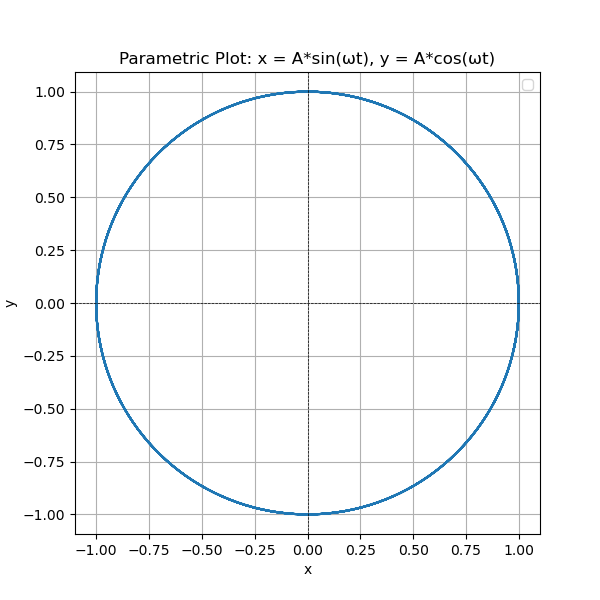
\includegraphics[width=\textwidth]{figs/Experiment-1/Observation-1/Figure_1.jpg}
        \caption{Actual plot of the equation}
    \end{subfigure}
    \hfill
    \begin{subfigure}[b]{0.45\textwidth}
        \centering
        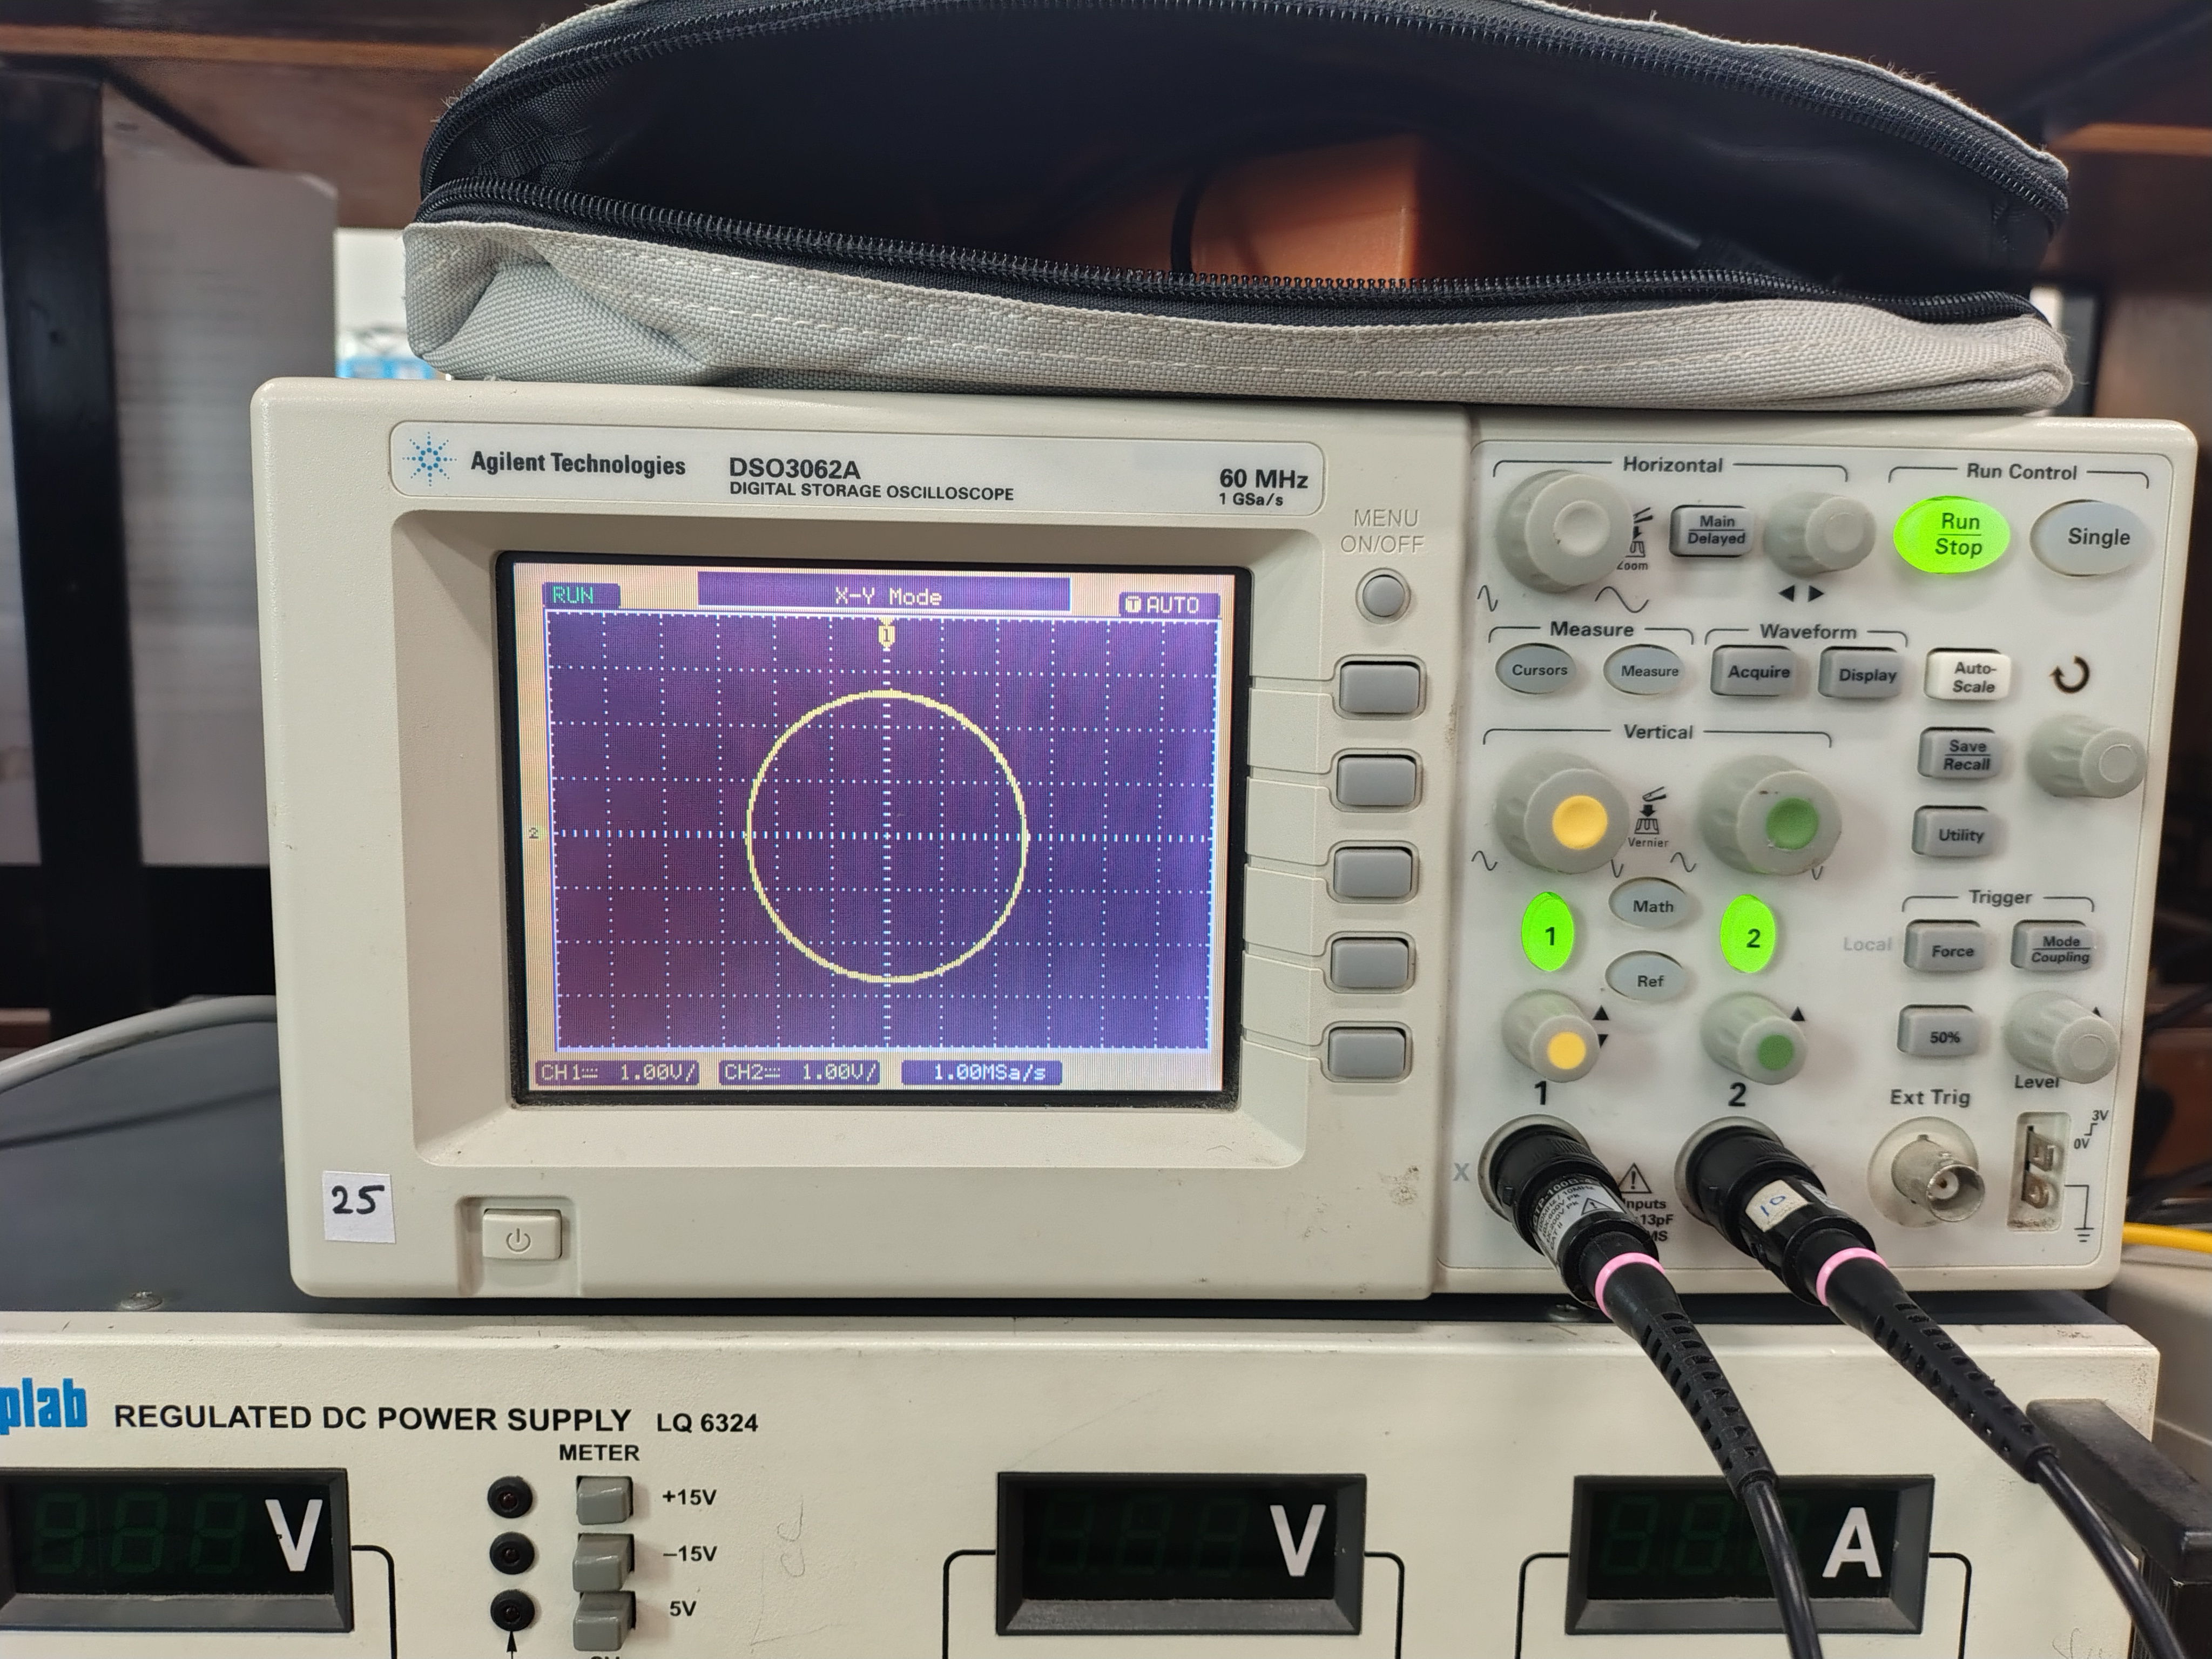
\includegraphics[width=\textwidth]{figs/Experiment-1/Observation-1/Figure_2.jpg}
        \caption{Figure obtained on the CRO}
    \end{subfigure}
    \caption{Pattern 1 - Circle}
\end{figure}

\subsection{Pattern 2:}
For the 2nd pattern, we set the following values:
\begin{table}[H]
    \centering
    \begin{tabular}{|c|c|c|}
    \hline
        & \textbf{Channel - 1} & \textbf{Channel - 2}\\
    \hline
    Frequency & 1.000 kHz & 1.000 kHz\\
    \hline
    Phase     & $0^{\circ}$ & $0^{\circ}$\\
    \hline
    High      & 2.500 V & 2.500 V\\
    \hline
    Low       & -2.500 V & -2.500 V\\
    \hline
    \end{tabular}
\end{table}

\textbf{Equation of Channel - 1} ($x$ - axis):
\[
x = A \sin{\left(\omega_1 t + \delta_1\right)}
\]
where $A$ = 5 Vpp, $\omega_1 = 2000 \pi \, rad s^{-1}$, $\delta_1 = 0^{\circ}$

\[
\implies x = A \sin{\left(\omega_1 t\right)}
\]

\textbf{Equation of Channel - 2} ($y$ - axis):
\[
y = A \sin{\left(\omega_2 t + \delta_2\right)}
\]
where $A$ = 5 Vpp, $\omega_2 = 2000 \pi \, rad s^{-1}$, $\delta_2 = 0^{\circ}$

\[
\implies y = A \sin{\left(\omega_2 t\right)}
\]

On solving these equations, we get:
\[
x = y
\]
These equations, when plotted, give a \textbf{straight line} pattern.

\begin{figure}[htbp]
    \centering
    \begin{subfigure}[b]{0.45\textwidth}
        \centering
        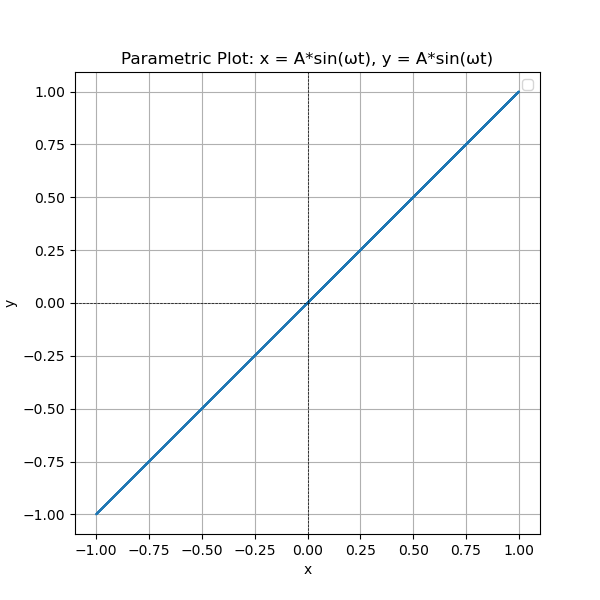
\includegraphics[width=\textwidth]{figs/Experiment-1/Observation-2/Figure_1.jpg}
        \caption{Actual plot of the equation}
    \end{subfigure}
    \hfill
    \begin{subfigure}[b]{0.45\textwidth}
        \centering
        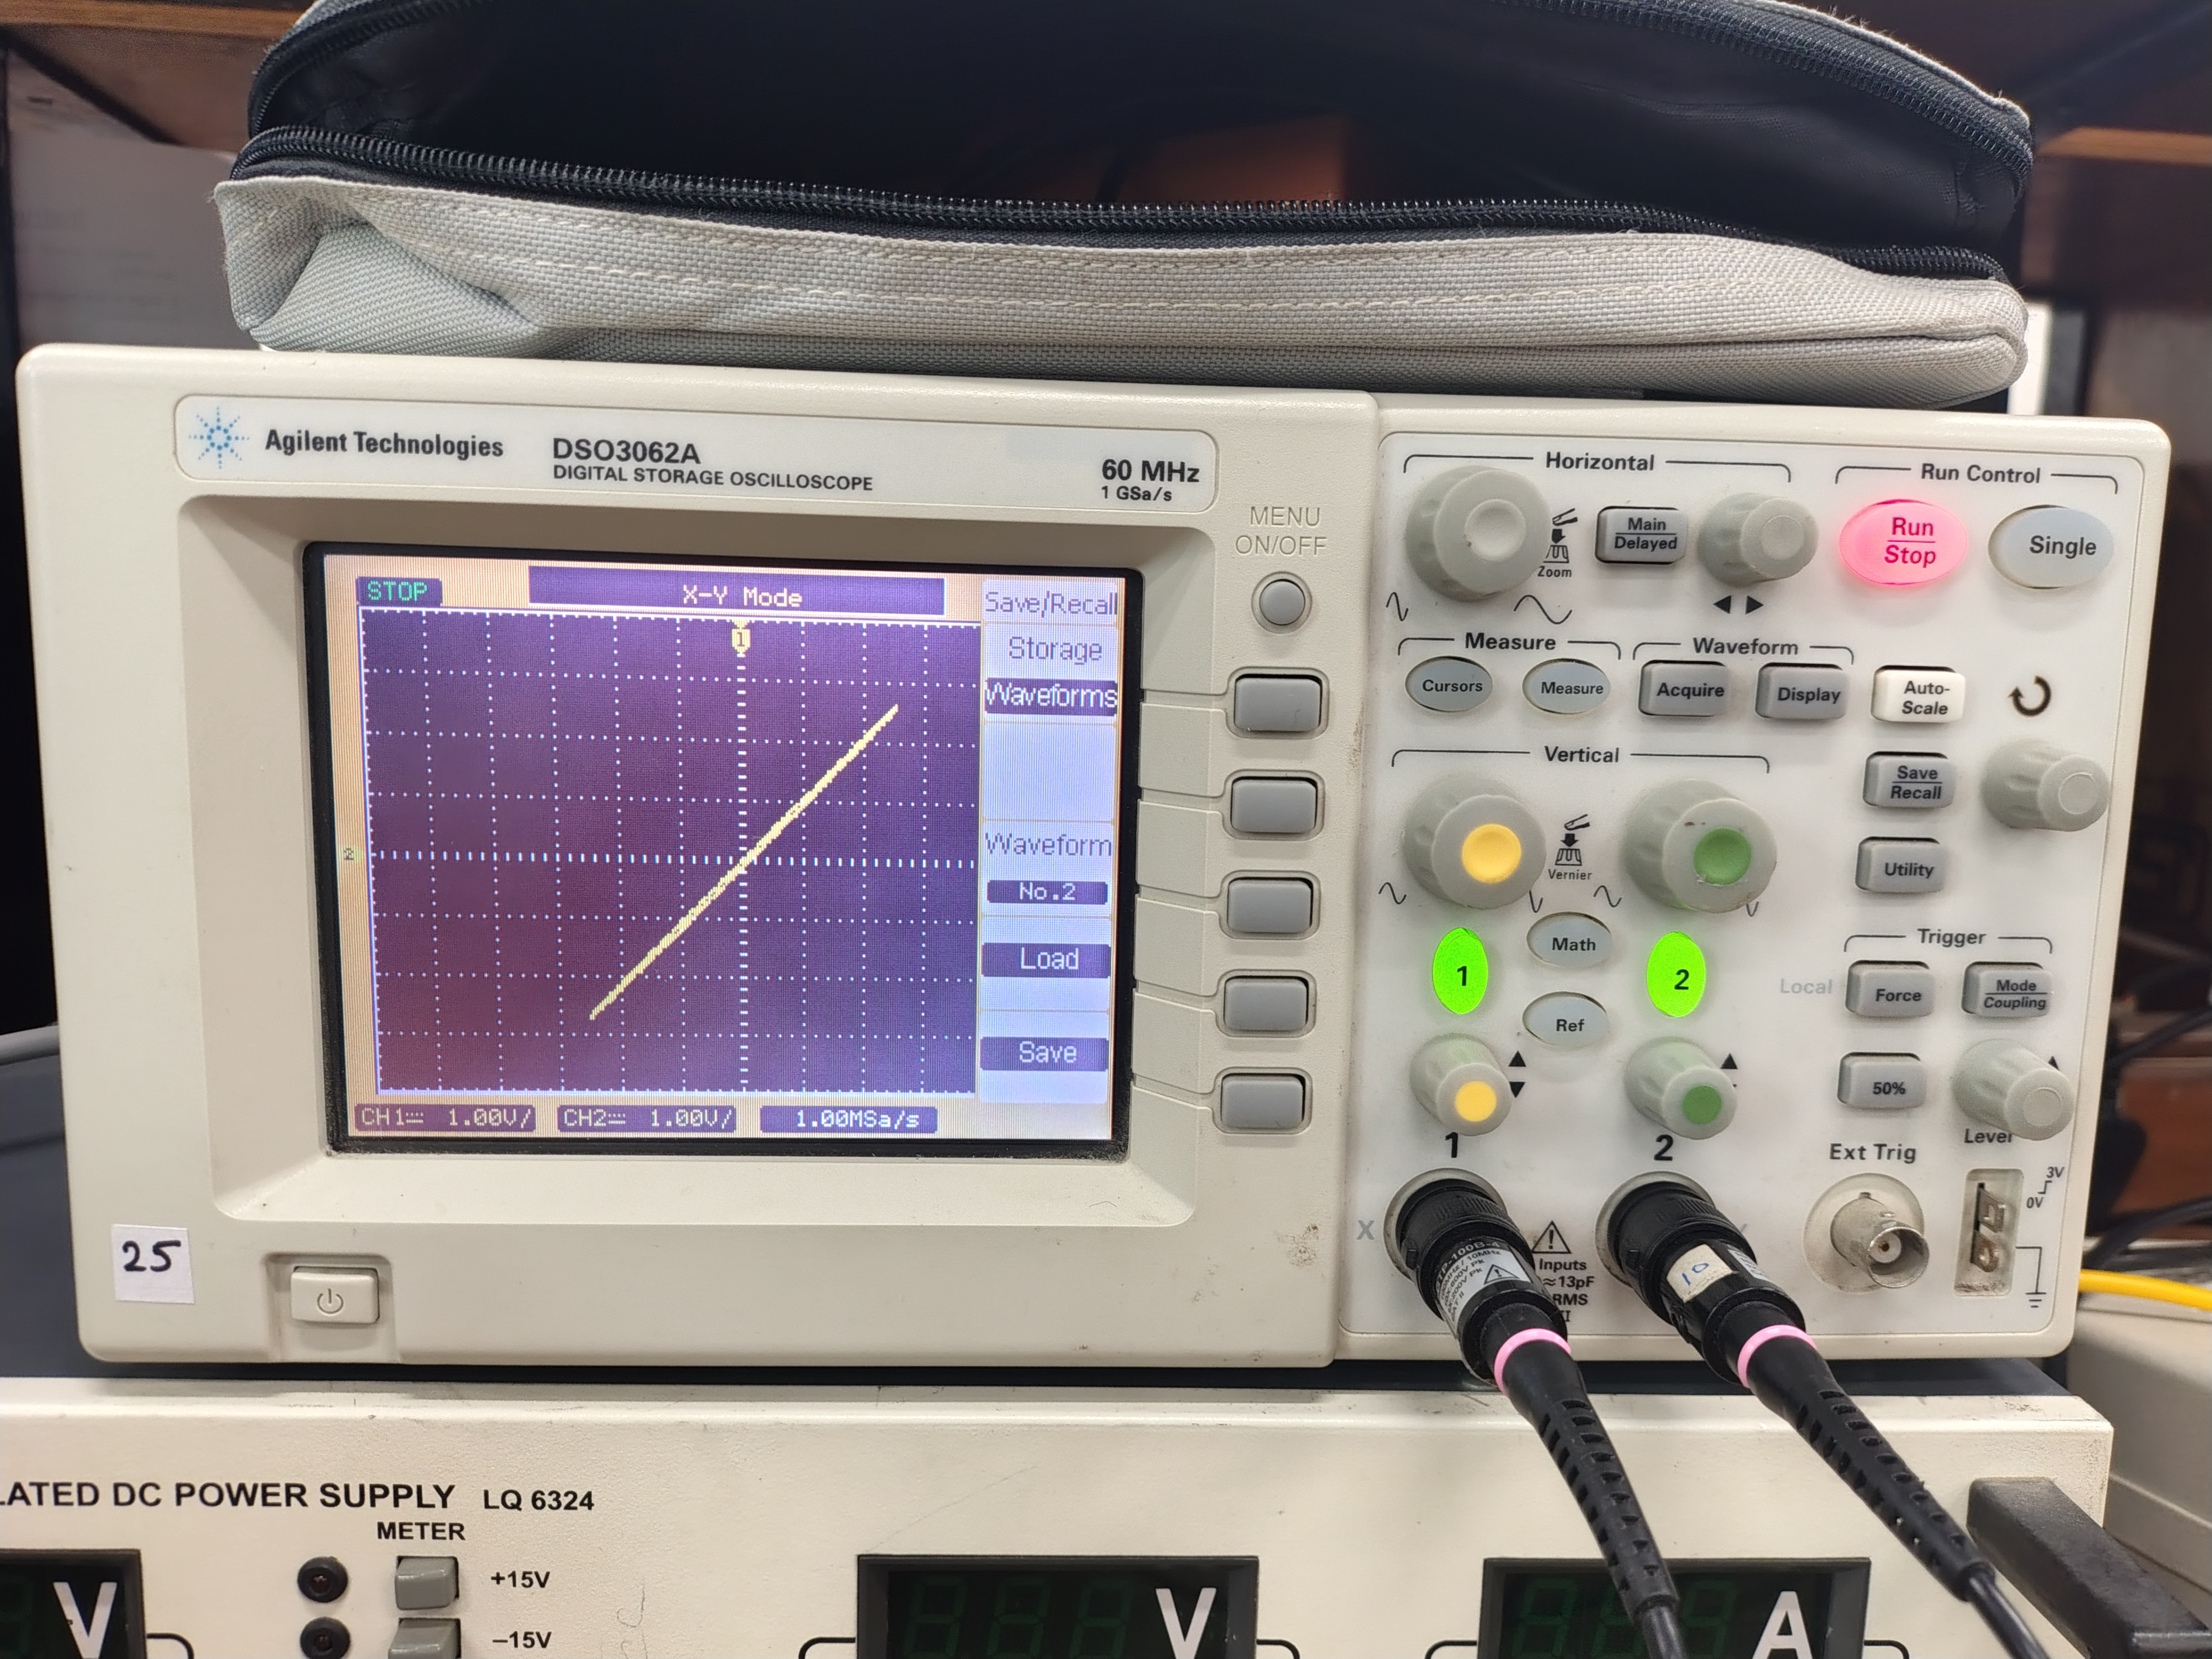
\includegraphics[width=\textwidth]{figs/Experiment-1/Observation-2/Figure_2.png}
        \caption{Figure obtained on the CRO}
    \end{subfigure}
    \caption{Pattern 2 - Straight Line}
\end{figure}

\subsection{Pattern 3:}
For the 3rd pattern, we set the following values:
\begin{table}[H]
    \centering
    \begin{tabular}{|c|c|c|}
    \hline
        & \textbf{Channel - 1} & \textbf{Channel - 2}\\
    \hline
    Frequency & 1.000 kHz & 1.000 kHz\\
    \hline
    Phase     & $0^{\circ}$ & $30^{\circ}$\\
    \hline
    High      & 2.500 V & 2.500 V\\
    \hline
    Low       & -2.500 V & -2.500 V\\
    \hline
    \end{tabular}
\end{table}

\textbf{Equation of Channel - 1} ($x$ - axis):
\[
x = A \sin{\left(\omega_1 t + \delta_1\right)}
\]
where $A$ = 5 Vpp, $\omega_1 = 2000 \pi \, rad s^{-1}$, $\delta_1 = 0^{\circ}$

\[
\implies x = A \sin{\left(\omega_1 t\right)}
\]

\textbf{Equation of Channel - 2} ($y$ - axis):
\[
y = A \sin{\left(\omega_2 t + \delta_2\right)}
\]
where $A$ = 5 Vpp, $\omega_2 = 2000 \pi \, rad s^{-1}$, $\delta_2 = 30^{\circ}$

\[
\implies y = A \sin{\left(\omega_2 t + 30^\circ\right)}
\]

On solving these equations, we get:
\[
\frac{x}{A} = \sin{\left(\omega t\right)}, \quad \frac{y}{A} = \sin{\left(\omega t + 30^\circ\right)}
\]
Using the trigonometric identity:
\[
\sin(a + b) = \sin(a)\cos(b) + \cos(a)\sin(b),
\]
\(y\) becomes:
\[
y = A \left( \frac{\sqrt{3}}{2} \sin(\omega t) + \frac{1}{2} \cos(\omega t) \right).
\]

From \(x = A \sin(\omega t)\), we find:
\[
\sin(\omega t) = \frac{x}{A}, \quad \cos(\omega t) = \pm \sqrt{1 - \left(\frac{x}{A}\right)^2}.
\]

Substitute these into \(y\):
\[
y = \frac{\sqrt{3}}{2}x \pm \frac{A}{2} \sqrt{1 - \left(\frac{x}{A}\right)^2}.
\]

Square both sides and simplify:
\[
\left(y - \frac{\sqrt{3}}{2}x\right)^2 = \frac{A^2}{4} - \frac{x^2}{4}.
\]

Rearrange to get the equation of an ellipse:
\[
\frac{x^2}{A^2} + \frac{\left(y - \frac{\sqrt{3}}{2}x\right)^2}{\frac{A^2}{4}} = 1.
\]

This confirms the parametric equations describe an ellipse.
This is the equation of an \textbf{ellipse}.

\begin{figure}[htbp]
    \centering
    \begin{subfigure}[b]{0.45\textwidth}
        \centering
        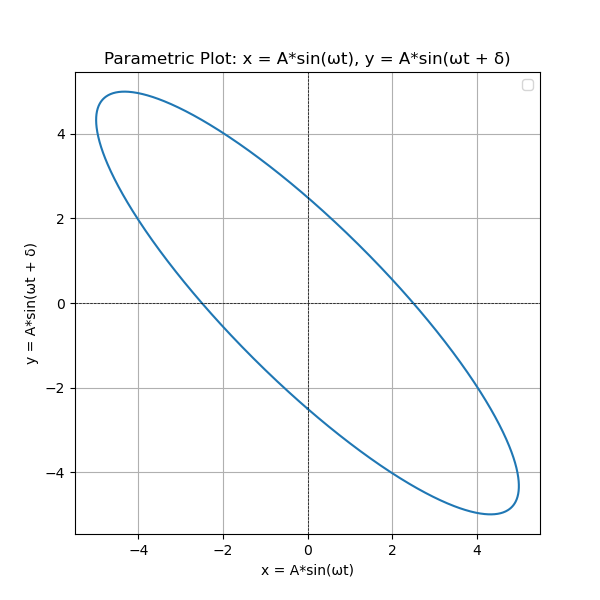
\includegraphics[width=\textwidth]{figs/Experiment-1/Observation-3/Figure_1.jpg}
        \caption{Actual plot of the equation}
    \end{subfigure}
    \hfill
    \begin{subfigure}[b]{0.45\textwidth}
        \centering
        \includegraphics[width=\textwidth]{figs/Experiment-1/Observation-3/Figure_2.png}
        \caption{Figure obtained on the CRO}
    \end{subfigure}
    \caption{Pattern 3 - Ellipse}
\end{figure}

\subsection{Pattern 4:}Pattern 4:
For the 4th pattern, we set the following values:
\begin{table}[H]
    \centering
    \begin{tabular}{|c|c|c|}
    \hline
        & \textbf{Channel - 1} & \textbf{Channel - 2}\\
    \hline
    Frequency & 1.000 kHz & 2.000 kHz\\
    \hline
    Phase     & $0^{\circ}$ & $30^{\circ}$\\
    \hline
    High      & 2.500 V & 2.500 V\\
    \hline
    Low       & -2.500 V & -2.500 V\\
    \hline
    \end{tabular}
\end{table}

\textbf{Equation of Channel - 1} ($x$ - axis):
\[
x = A \sin{\left(\omega_1 t + \delta_1\right)}
\]
where $A$ = 5 Vpp, $\omega_1 = 2000 \pi \, rad s^{-1}$, $\delta_1 = 0^{\circ}$

\[
\implies x = A \sin{\left(\omega_1 t\right)}
\]

\textbf{Equation of Channel - 2} ($y$ - axis):
\[
y = A \sin{\left(\omega_2 t + \delta_2\right)}
\]
where $A$ = 5 Vpp, $\omega_2 = 4000 \pi \, rad s^{-1}$, $\delta_2 = 30^{\circ}$

\[
\implies y = A \sin{\left(\omega_2 t + 30^\circ\right)}
\]

On solving these equations, we get:
\[
x = A \sin{\left(\omega t\right)}, \quad y = A \sin{\left(2 \omega t + 30^\circ\right)}
\]


Using the angle addition formula:

\[
\sin(2\omega t + 30^\circ) = \sin(2\omega t)\cos 30^\circ + \cos(2\omega t)\sin 30^\circ
\]

Since \( \cos 30^\circ = \frac{\sqrt{3}}{2} \) and \( \sin 30^\circ = \frac{1}{2} \), we get:

\[
\sin(2\omega t + 30^\circ) = \frac{\sqrt{3}}{2} \sin(2\omega t) + \frac{1}{2} \cos(2\omega t)
\]

Using the double-angle identities:

\[
\sin(2\omega t) = 2 \sin(\omega t)\cos(\omega t)
\]
\[
\cos(2\omega t) = 1 - 2\sin^2(\omega t)
\]

Substituting these identities:

\[
y = \sqrt{3} x \sqrt{1 - \frac{x^2}{A^2}} + \frac{A}{2} - \frac{x^2}{A}
\]

These equations, when plotted, give a Lissajous Figure with more complexity and variation which can be verified using Python script

\begin{figure}[htbp]
    \centering
    \begin{subfigure}[b]{0.45\textwidth}
        \centering
        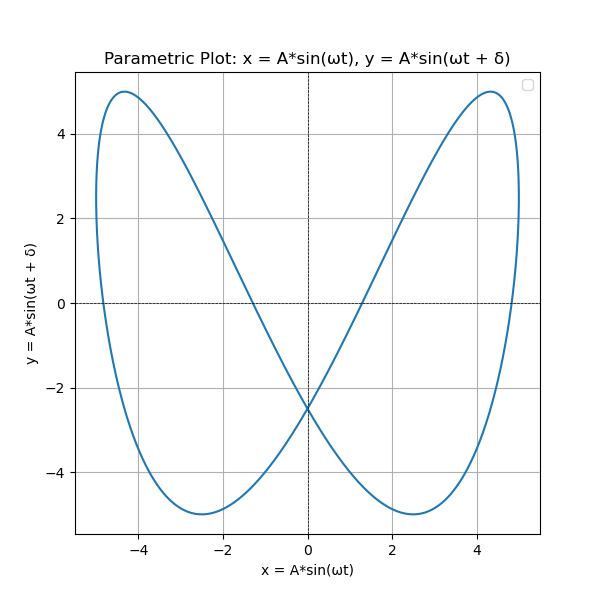
\includegraphics[width=\textwidth]{figs/Experiment-1/Observation-4/Figure_1.jpg}
        \caption{Actual plot of the equation}
    \end{subfigure}
    \hfill
    \begin{subfigure}[b]{0.45\textwidth}
        \centering
        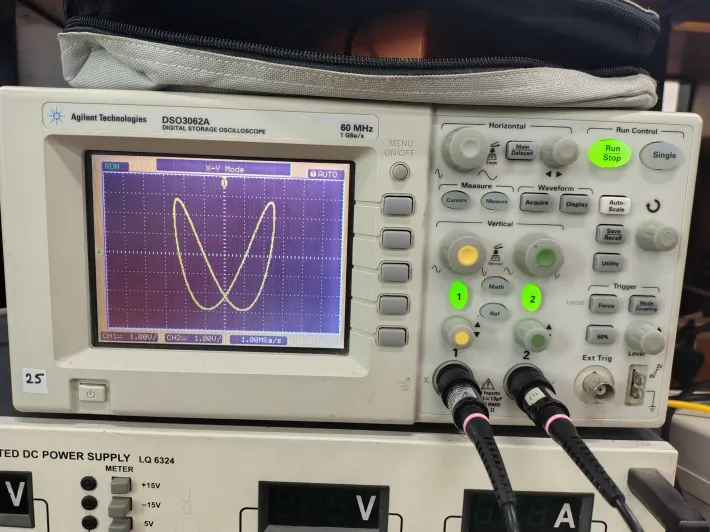
\includegraphics[width=\textwidth]{figs/Experiment-1/Observation-4/Figure_2.png}
        \caption{Figure obtained on the CRO}
    \end{subfigure}
    \caption{Pattern 4 - Complex Lissajous Curve}
\end{figure}

\subsection{Pattern 5:}
For the 5th pattern, we set the following values:
\begin{table}[H]
    \centering
    \begin{tabular}{|c|c|c|}
    \hline
        & \textbf{Channel - 1} & \textbf{Channel - 2}\\
    \hline
    Frequency & 1.000 kHz & 2.000 kHz\\
    \hline
    Phase     & $0^{\circ}$ & $90^{\circ}$\\
    \hline
    High      & 2.500 V & 2.500 V\\
    \hline
    Low       & -2.500 V & -2.500 V\\
    \hline
    \end{tabular}
\end{table}

\textbf{Equation of Channel - 1} ($x$ - axis):
\[
x = A \sin{\left(\omega_1 t + \delta_1\right)}
\]
where $A$ = 5 Vpp, $\omega_1 = 2000 \pi \, rad s^{-1}$, $\delta_1 = 0^{\circ}$

\[
\implies x = A \sin{\left(\omega_1 t\right)}
\]

\textbf{Equation of Channel - 2} ($y$ - axis):
\[
y = A \sin{\left(\omega_2 t + \delta_2\right)}
\]
where $A$ = 5 Vpp, $\omega_2 = 4000 \pi \, rad s^{-1}$, $\delta_2 = 90^{\circ}$

\[
\implies y = A \sin{\left(\omega_2 t + 90^\circ\right)}
\]

On solving these equations, we get:
\[
x = A \sin{\left(\omega t\right)}, \quad y = A \sin{\left(2 \omega t + 90^\circ\right)}
\]

Since \( \sin(2\omega t + 90^\circ) = \cos(2\omega t) \), the equation for \( y \) becomes:

\[
y = A \cos(2\omega t)
\]

Using the double-angle identity:

\[
\cos(2\omega t) = 1 - 2\sin^2(\omega t)
\]

Substituting \( \sin(\omega t) = \frac{x}{A} \):

\[
y = A \left(1 - 2 \frac{x^2}{A^2}\right)
\]

\[
y = A - \frac{2x^2}{A}
\]
These equations, when plotted, give a Lissajous Figure with more complexity and variation which can be verified using Python script

\begin{figure}[htbp]
    \centering
    \begin{subfigure}[b]{0.45\textwidth}
        \centering
        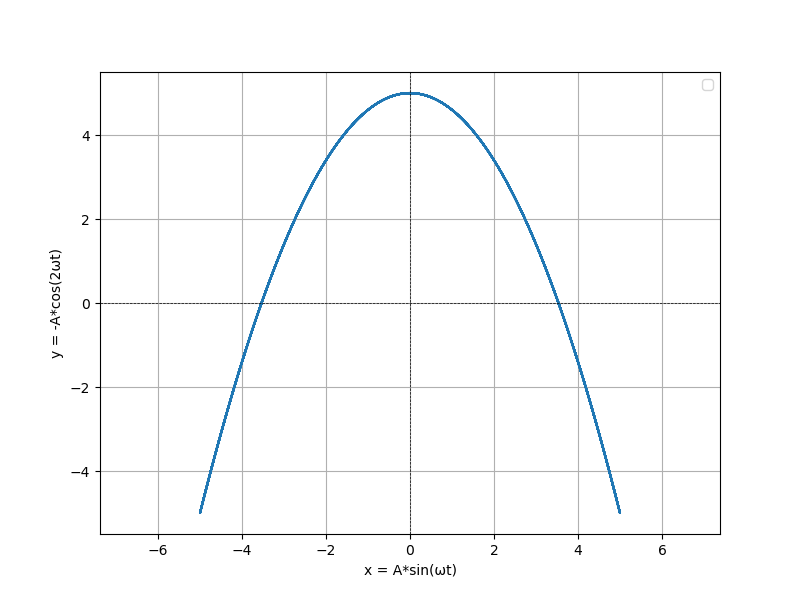
\includegraphics[width=\textwidth]{figs/Experiment-1/Observation-5/Figure_1.jpg}
        \caption{Actual plot of the equation}
    \end{subfigure}
    \hfill
    \begin{subfigure}[b]{0.45\textwidth}
        \centering
        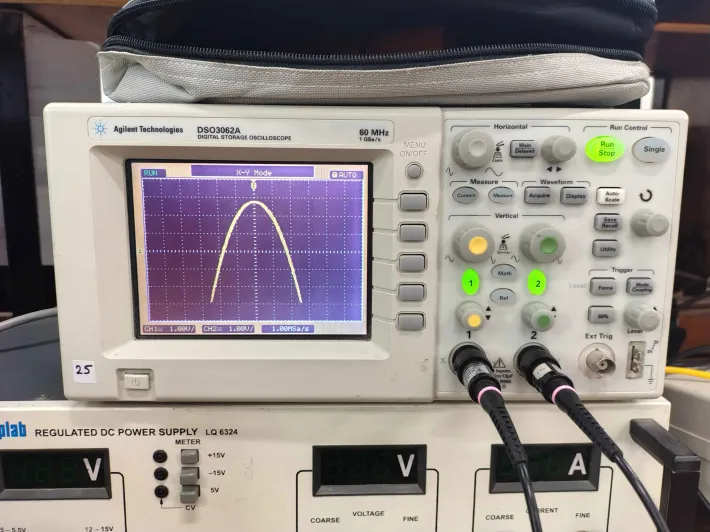
\includegraphics[width=\textwidth]{figs/Experiment-1/Observation-5/Figure_2.png}
        \caption{Figure obtained on the CRO}
    \end{subfigure}
    \caption{Pattern 5 - Moderate Lissajous Curve}
\end{figure}

\subsection{Pattern 6:}
For the 6th pattern, we set the following values:
\begin{table}[H]
    \centering
    \begin{tabular}{|c|c|c|}
    \hline
        & \textbf{Channel - 1} & \textbf{Channel - 2}\\
    \hline
    Frequency & 3.000 kHz & 2.000 kHz\\
    \hline
    Phase     & $0^{\circ}$ & $0^{\circ}$\\
    \hline
    High      & 2.500 V & 2.500 V\\
    \hline
    Low       & -2.500 V & -2.500 V\\
    \hline
    \end{tabular}
\end{table}

\textbf{Equation of Channel - 1} ($x$ - axis):
\[
x = A \sin{\left(\omega_1 t + \delta_1\right)}
\]
where $A$ = 5 Vpp, $\omega_1 = 6000 \pi \, rad s^{-1}$, $\delta_1 = 0^{\circ}$

\[
\implies x = A \sin{\left(\omega_1 t\right)}
\]

\textbf{Equation of Channel - 2} ($y$ - axis):
\[
y = A \sin{\left(\omega_2 t + \delta_2\right)}
\]
where $A$ = 5 Vpp, $\omega_2 = 4000 \pi \, rad s^{-1}$, $\delta_2 = 0^{\circ}$

\[
\implies y = A \sin{\left(\omega_2 t\right)}
\]

On solving these equations, we get:
\[
x = A \sin{\left(1.5\omega t\right)}, \quad y = A \sin{\left(\omega t\right)}
\]

From the second equation, \( y = A \sin(\omega t) \), we have:
\[
\sin(\omega t) = \frac{y}{A}.
\]

Using the angle-sum identity for sine:
\[
\sin(1.5\omega t) = \sin(\omega t + 0.5\omega t) = \sin(\omega t)\cos(0.5\omega t) + \cos(\omega t)\sin(0.5\omega t),
\]
we substitute \( \sin(\omega t) = \frac{y}{A} \) into this:
\[
\sin(1.5\omega t) = \frac{y}{A}\cos(0.5\omega t) + \cos(\omega t)\sin(0.5\omega t).
\]

Now, using the identity \( \sin^2(\omega t) + \cos^2(\omega t) = 1 \), we find:
\[
\cos^2(\omega t) = 1 - \sin^2(\omega t),
\]
so:
\[
\cos(\omega t) = \pm \sqrt{1 - \frac{y^2}{A^2}}.
\]

Next, using the half-angle identities:
\[
\cos(0.5\omega t) = \pm \sqrt{\frac{1 + \cos(\omega t)}{2}}, \quad \sin(0.5\omega t) = \pm \sqrt{\frac{1 - \cos(\omega t)}{2}},
\]
we substitute \( \cos(\omega t) = \pm \sqrt{1 - \frac{y^2}{A^2}} \) into these:
\[
\cos(0.5\omega t) = \pm \sqrt{\frac{1 + \sqrt{1 - \frac{y^2}{A^2}}}{2}}, \quad \sin(0.5\omega t) = \pm \sqrt{\frac{1 - \sqrt{1 - \frac{y^2}{A^2}}}{2}}.
\]

Substituting \( \sin(\omega t) \), \( \cos(\omega t) \), \( \cos(0.5\omega t) \), and \( \sin(0.5\omega t) \) into \( x = A \sin(1.5\omega t) \), we get:
\[
x = A \left( \frac{y}{A}\cos(0.5\omega t) + \cos(\omega t)\sin(0.5\omega t) \right).
\]

This simplifies to:
\[
x = A \left[ \frac{y}{A} \cdot \pm \sqrt{\frac{1 + \sqrt{1 - \frac{y^2}{A^2}}}{2}} + \pm \sqrt{1 - \frac{y^2}{A^2}} \cdot \pm \sqrt{\frac{1 - \sqrt{1 - \frac{y^2}{A^2}}}{2}} \right].
\]

Squaring both sides to remove the square roots results in a complex expression that can be simplified further. However, due to the involvement of multiple nested square roots, the resulting equation is non-trivial and is better represented as a polynomial in \( y \) and \( A \).


These equations, when plotted, give a Lissajous Figure with more complexity and variation which can be verified using Python script
\begin{figure}[htbp]
    \centering
    \begin{subfigure}[b]{0.45\textwidth}
        \centering
        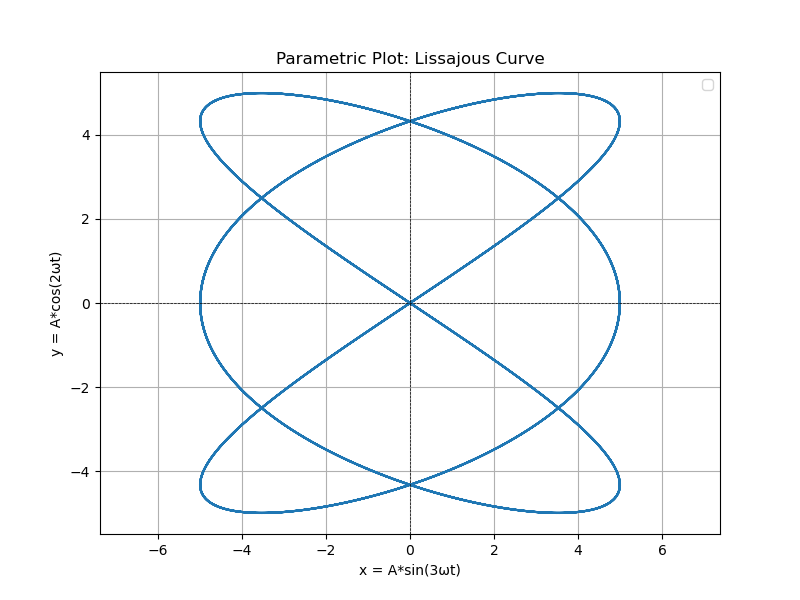
\includegraphics[width=\textwidth]{figs/Experiment-1/Observation-6/Figure_1.jpg}
        \caption{Actual plot of the equation}
    \end{subfigure}
    \hfill
    \begin{subfigure}[b]{0.45\textwidth}
        \centering
        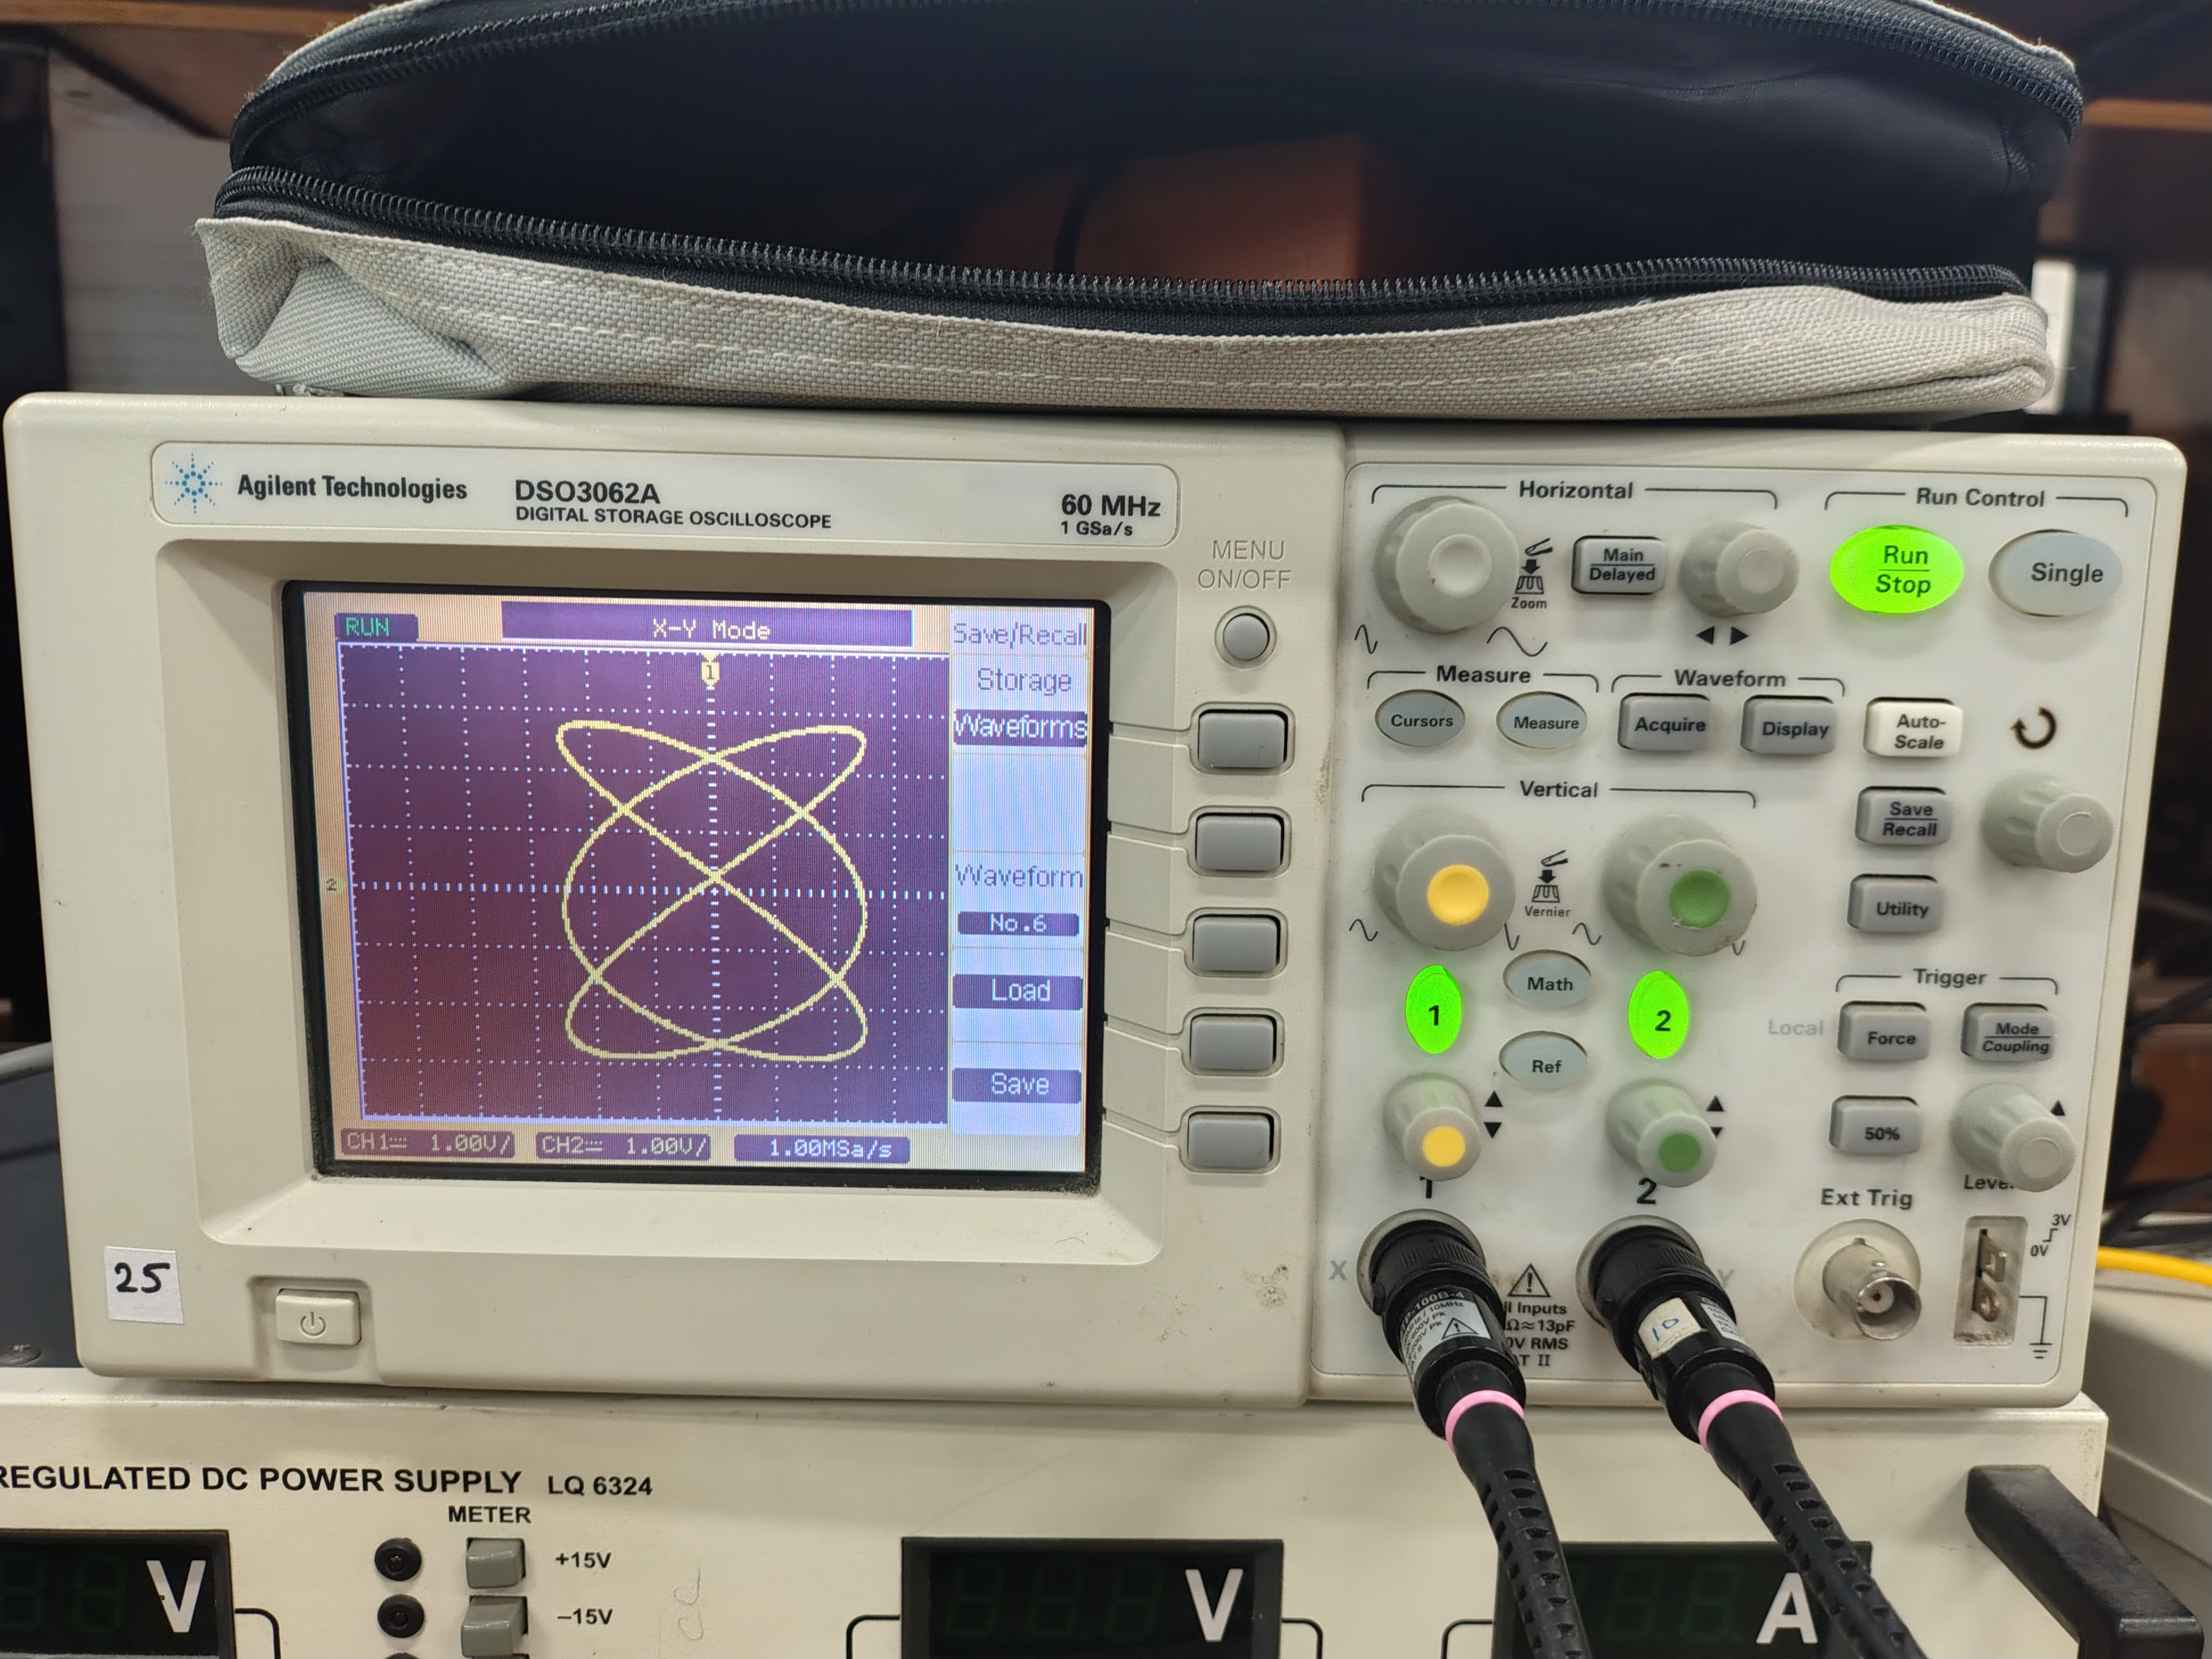
\includegraphics[width=\textwidth]{figs/Experiment-1/Observation-6/Figure_2.png}
        \caption{Figure obtained on the CRO}
    \end{subfigure}
    \caption{Pattern 6 - Lissajous Curve}
\end{figure}


\subsection{Pattern 7:}
For the 7th pattern, we set the following values:
\begin{table}[H]
    \centering
    \begin{tabular}{|c|c|c|}
    \hline
        & \textbf{Channel - 1} & \textbf{Channel - 2}\\
    \hline
    Frequency & 2.000 kHz & 1.000 kHz\\
    \hline
    Phase     & $0^{\circ}$ & $0^{\circ}$\\
    \hline
    High      & 2.500 V & 2.500 V\\
    \hline
    Low       & -2.500 V & -2.500 V\\
    \hline
    \end{tabular}
\end{table}

\textbf{Equation of Channel - 1} ($x$ - axis):
\[
x = A \sin{\left(\omega_1 t + \delta_1\right)}
\]
where $A$ = 5 Vpp, $\omega_1 = 4000 \pi \, rad s^{-1}$, $\delta_1 = 0^{\circ}$

\[
\implies x = A \sin{\left(\omega_1 t\right)}
\]

\textbf{Equation of Channel - 2} ($y$ - axis):
\[
y = A \sin{\left(\omega_2 t + \delta_2\right)}
\]
where $A$ = 5 Vpp, $\omega_2 = 2000 \pi \, rad s^{-1}$, $\delta_2 = 0^{\circ}$

\[
\implies y = A \sin{\left(\omega_2 t\right)}
\]

On solving these equations, we get:
\[
x = A \sin{\left( 2\omega t\right)}, \quad y = A \cos{\left(\omega t\right)}
\]


Using the double-angle identity for sine:
\[
\sin(2\omega t) = 2\sin(\omega t)\cos(\omega t),
\]
we substitute this into \( x \) to get:
\[
x = 2A \sin(\omega t)\cos(\omega t).
\]

From the second equation, \( y = A \cos(\omega t) \), we can express:
\[
\cos(\omega t) = \frac{y}{A}.
\]

Using the Pythagorean identity:
\[
\sin^2(\omega t) + \cos^2(\omega t) = 1,
\]
we find:
\[
\sin^2(\omega t) = 1 - \cos^2(\omega t).
\]
Substituting \( \cos(\omega t) = \frac{y}{A} \), we have:
\[
\sin^2(\omega t) = 1 - \frac{y^2}{A^2}.
\]
Taking the square root gives:
\[
\sin(\omega t) = \pm \sqrt{1 - \frac{y^2}{A^2}}.
\]

Substituting \( \sin(\omega t) \) and \( \cos(\omega t) \) into \( x = 2A \sin(\omega t)\cos(\omega t) \), we obtain:
\[
x = 2A \left( \pm \sqrt{1 - \frac{y^2}{A^2}} \right) \cdot \frac{y}{A}.
\]
Simplifying:
\[
x = \pm 2 \sqrt{1 - \frac{y^2}{A^2}} \cdot y.
\]

Squaring both sides to remove the square root:
\[
x^2 = 4 \left( 1 - \frac{y^2}{A^2} \right) y^2.
\]
Expanding:
\[
x^2 = 4y^2 - \frac{4y^4}{A^2}.
\]
Multiplying through by \( A^2 \) to eliminate the denominator:
\[
A^2 x^2 = 4A^2 y^2 - 4y^4.
\]
Rearranging terms:
\[
4y^4 - 4A^2 y^2 + A^2 x^2 = 0.
\]

Thus, the equation of the curve is:
\[
4y^4 - 4A^2 y^2 + A^2 x^2 = 0.
\]

These equations, when plotted, give a Lissajous Figure with more complexity and variation which can be verified using Python script
\begin{figure}[htbp]
    \centering
    \begin{subfigure}[b]{0.45\textwidth}
        \centering
        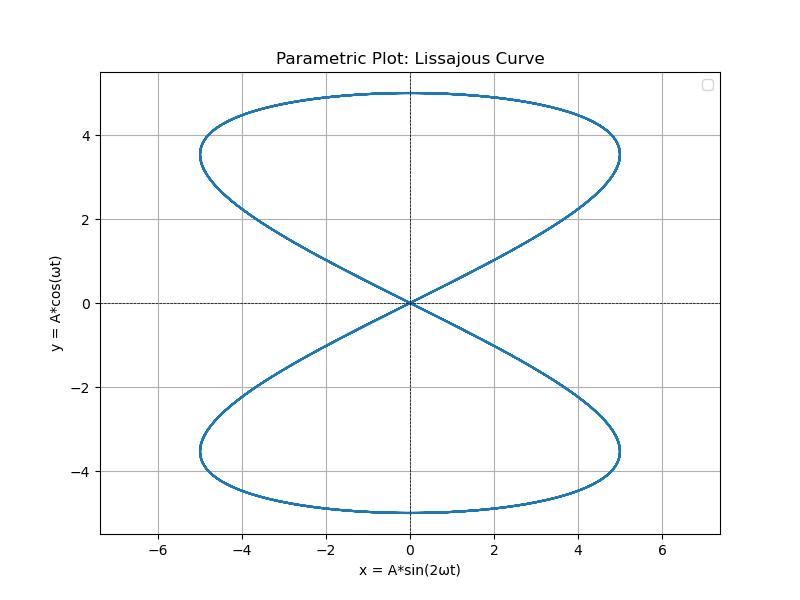
\includegraphics[width=\textwidth]{figs/Experiment-1/Observation-7/Figure_1.jpg}
        \caption{Actual plot of the equation}
    \end{subfigure}
    \hfill
    \begin{subfigure}[b]{0.45\textwidth}
        \centering
        \includegraphics[width=\textwidth]{figs/Experiment-1/Observation-7/Figure_2.png}
        \caption{Figure obtained on the CRO}
    \end{subfigure}
    \caption{Pattern 7 - Lissajous Curve}
\end{figure}


\section{Capturing One-time event in an oscilloscope(Task-2)}
\subsection{What is one-time event:}
\begin{itemize}
\item A one-time event is a phenomenon or signal that occurs only once or for a brief duration without repetition. These events are transient and do not have a repetitive pattern, making them difficult to capture unless the instrument is specifically set up to do so.\\
\end{itemize}
\subsection{How to Capture a One-Time Event on an Oscilloscope}

This document explains the process of capturing a one-time event on an oscilloscope using a function generator in burst mode. The aim is to ensure accurate measurement and visualization of the transient response.
\section*{Instruments Required}
The following instruments are required for this experiment:
\begin{itemize}
    \item \textbf{Oscilloscope}: To capture and display the one-time waveform.
    \item \textbf{Function Generator}: To generate the desired pulse waveform in burst mode.
    \item \textbf{Connecting Cables}: To connect the function generator to the oscilloscope.
    \item \textbf{Probes}: To ensure proper transmission of signals between devices.
\end{itemize}
\section*{Procedure}
The experiment involves the following steps:

\begin{enumerate}
    \item \textbf{Setup the Oscilloscope:}
    \begin{itemize}
        \item Set the oscilloscope's trigger sweep mode to \textit{Normal}.
        \item Adjust the trigger level to a value slightly less than the expected amplitude of the waveform. This ensures the oscilloscope triggers properly when the event occurs.
    \end{itemize}
    
    \item \textbf{Configure the Function Generator:}
    \begin{itemize}
        \item Select the \textit{Pulse} waveform option on the function generator.
        \item Enable \textit{Burst Mode} on the function generator.
        \item Set the trigger mode of the function generator to \textit{Manual}.
        \item Configure the burst mode to output a pulse train with \textbf{10 cycles}.
    \end{itemize}
    
    \item \textbf{Prepare the Oscilloscope for Single Capture:}
    \begin{itemize}
        \item Switch the oscilloscope to \textit{Single Mode}. This mode allows the oscilloscope to capture and store a one-time event for later analysis.
    \end{itemize}
    
    \item \textbf{Capture the Waveform:}
    \begin{itemize}
        \item Push the waveform from the function generator to the oscilloscope by pressing the \textit{Manual Trigger} button on the function generator.
        \item The oscilloscope will capture the event and display the waveform corresponding to the 10 cycles generated by the function generator.
    \end{itemize}
\end{enumerate}
\subsection{Snapshots of Capturing one-time event}
To provide evidence and further understanding of the experiment, snapshots of the oscilloscope and function generator are included below.
\subsection*{Oscilloscope Snapshot}
\begin{figure}[H]
    \centering
    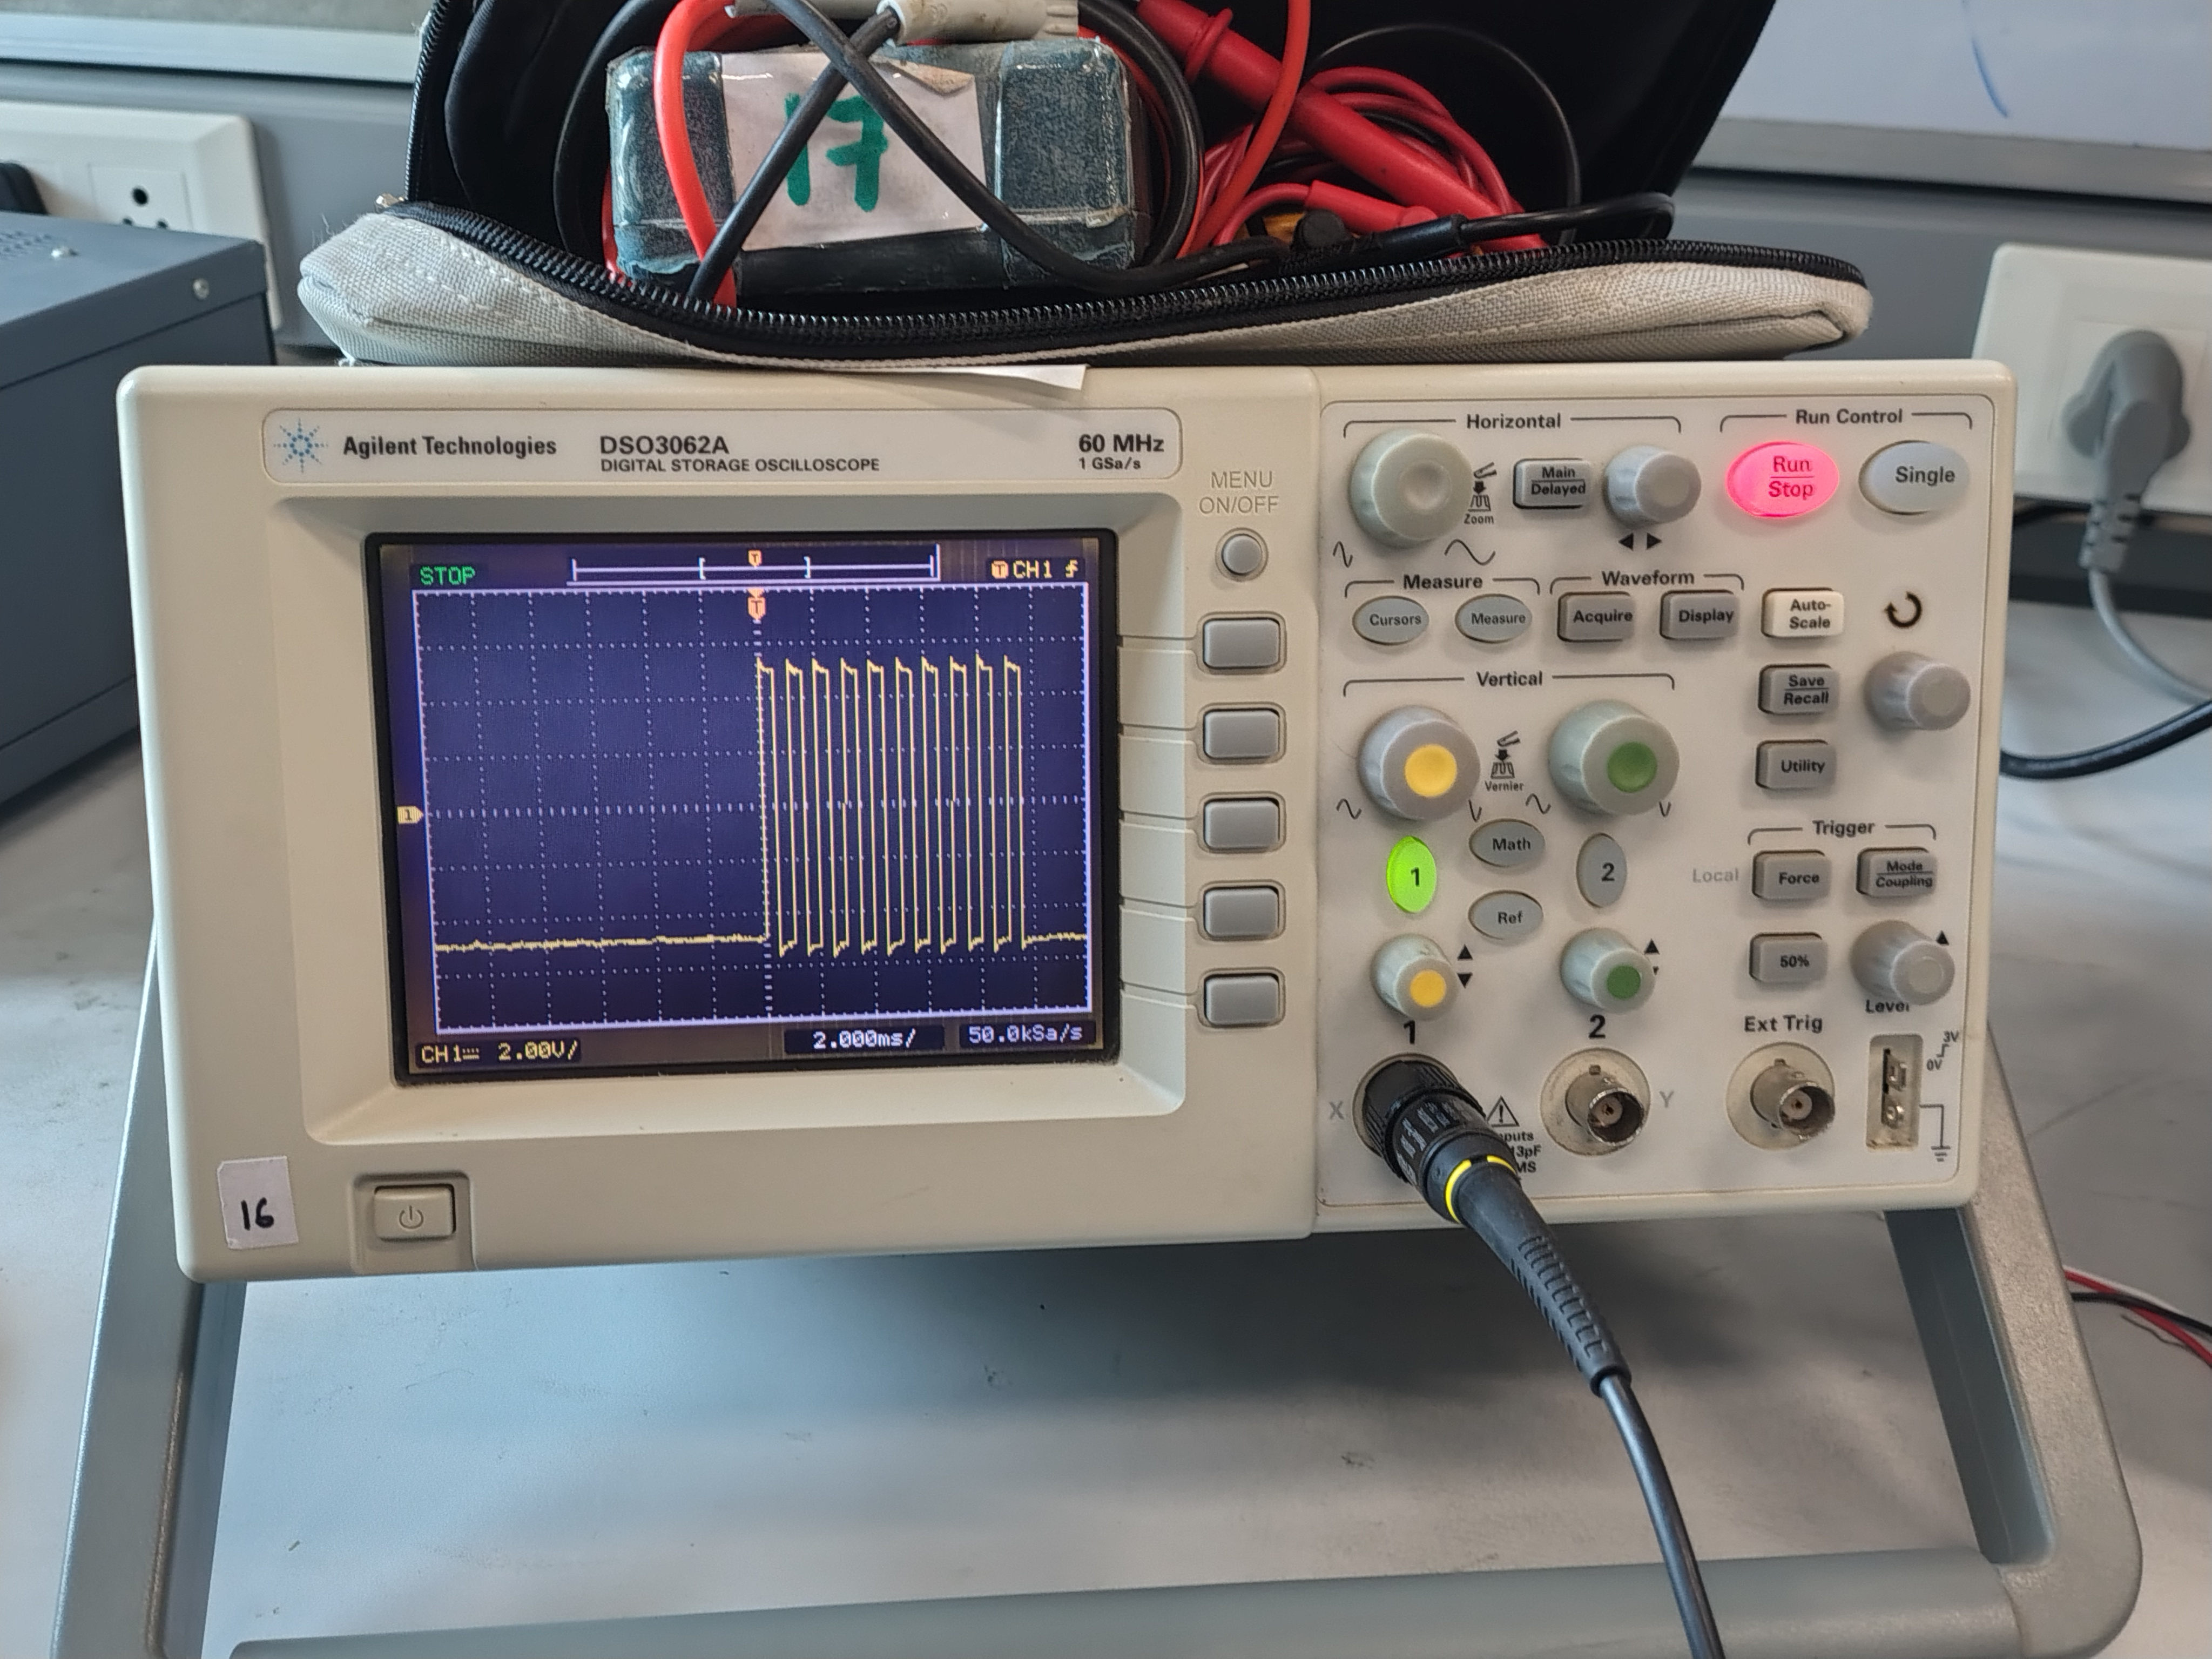
\includegraphics[width=0.7\textwidth]{figs/Experiment-2/1.2.1.jpg}
    \caption{Captured waveform on the oscilloscope showing the 10-cycle pulse train.}
    \label{fig:oscilloscope}
\end{figure}

\subsection*{Function Generator Snapshot}
\begin{figure}[H]
    \centering
    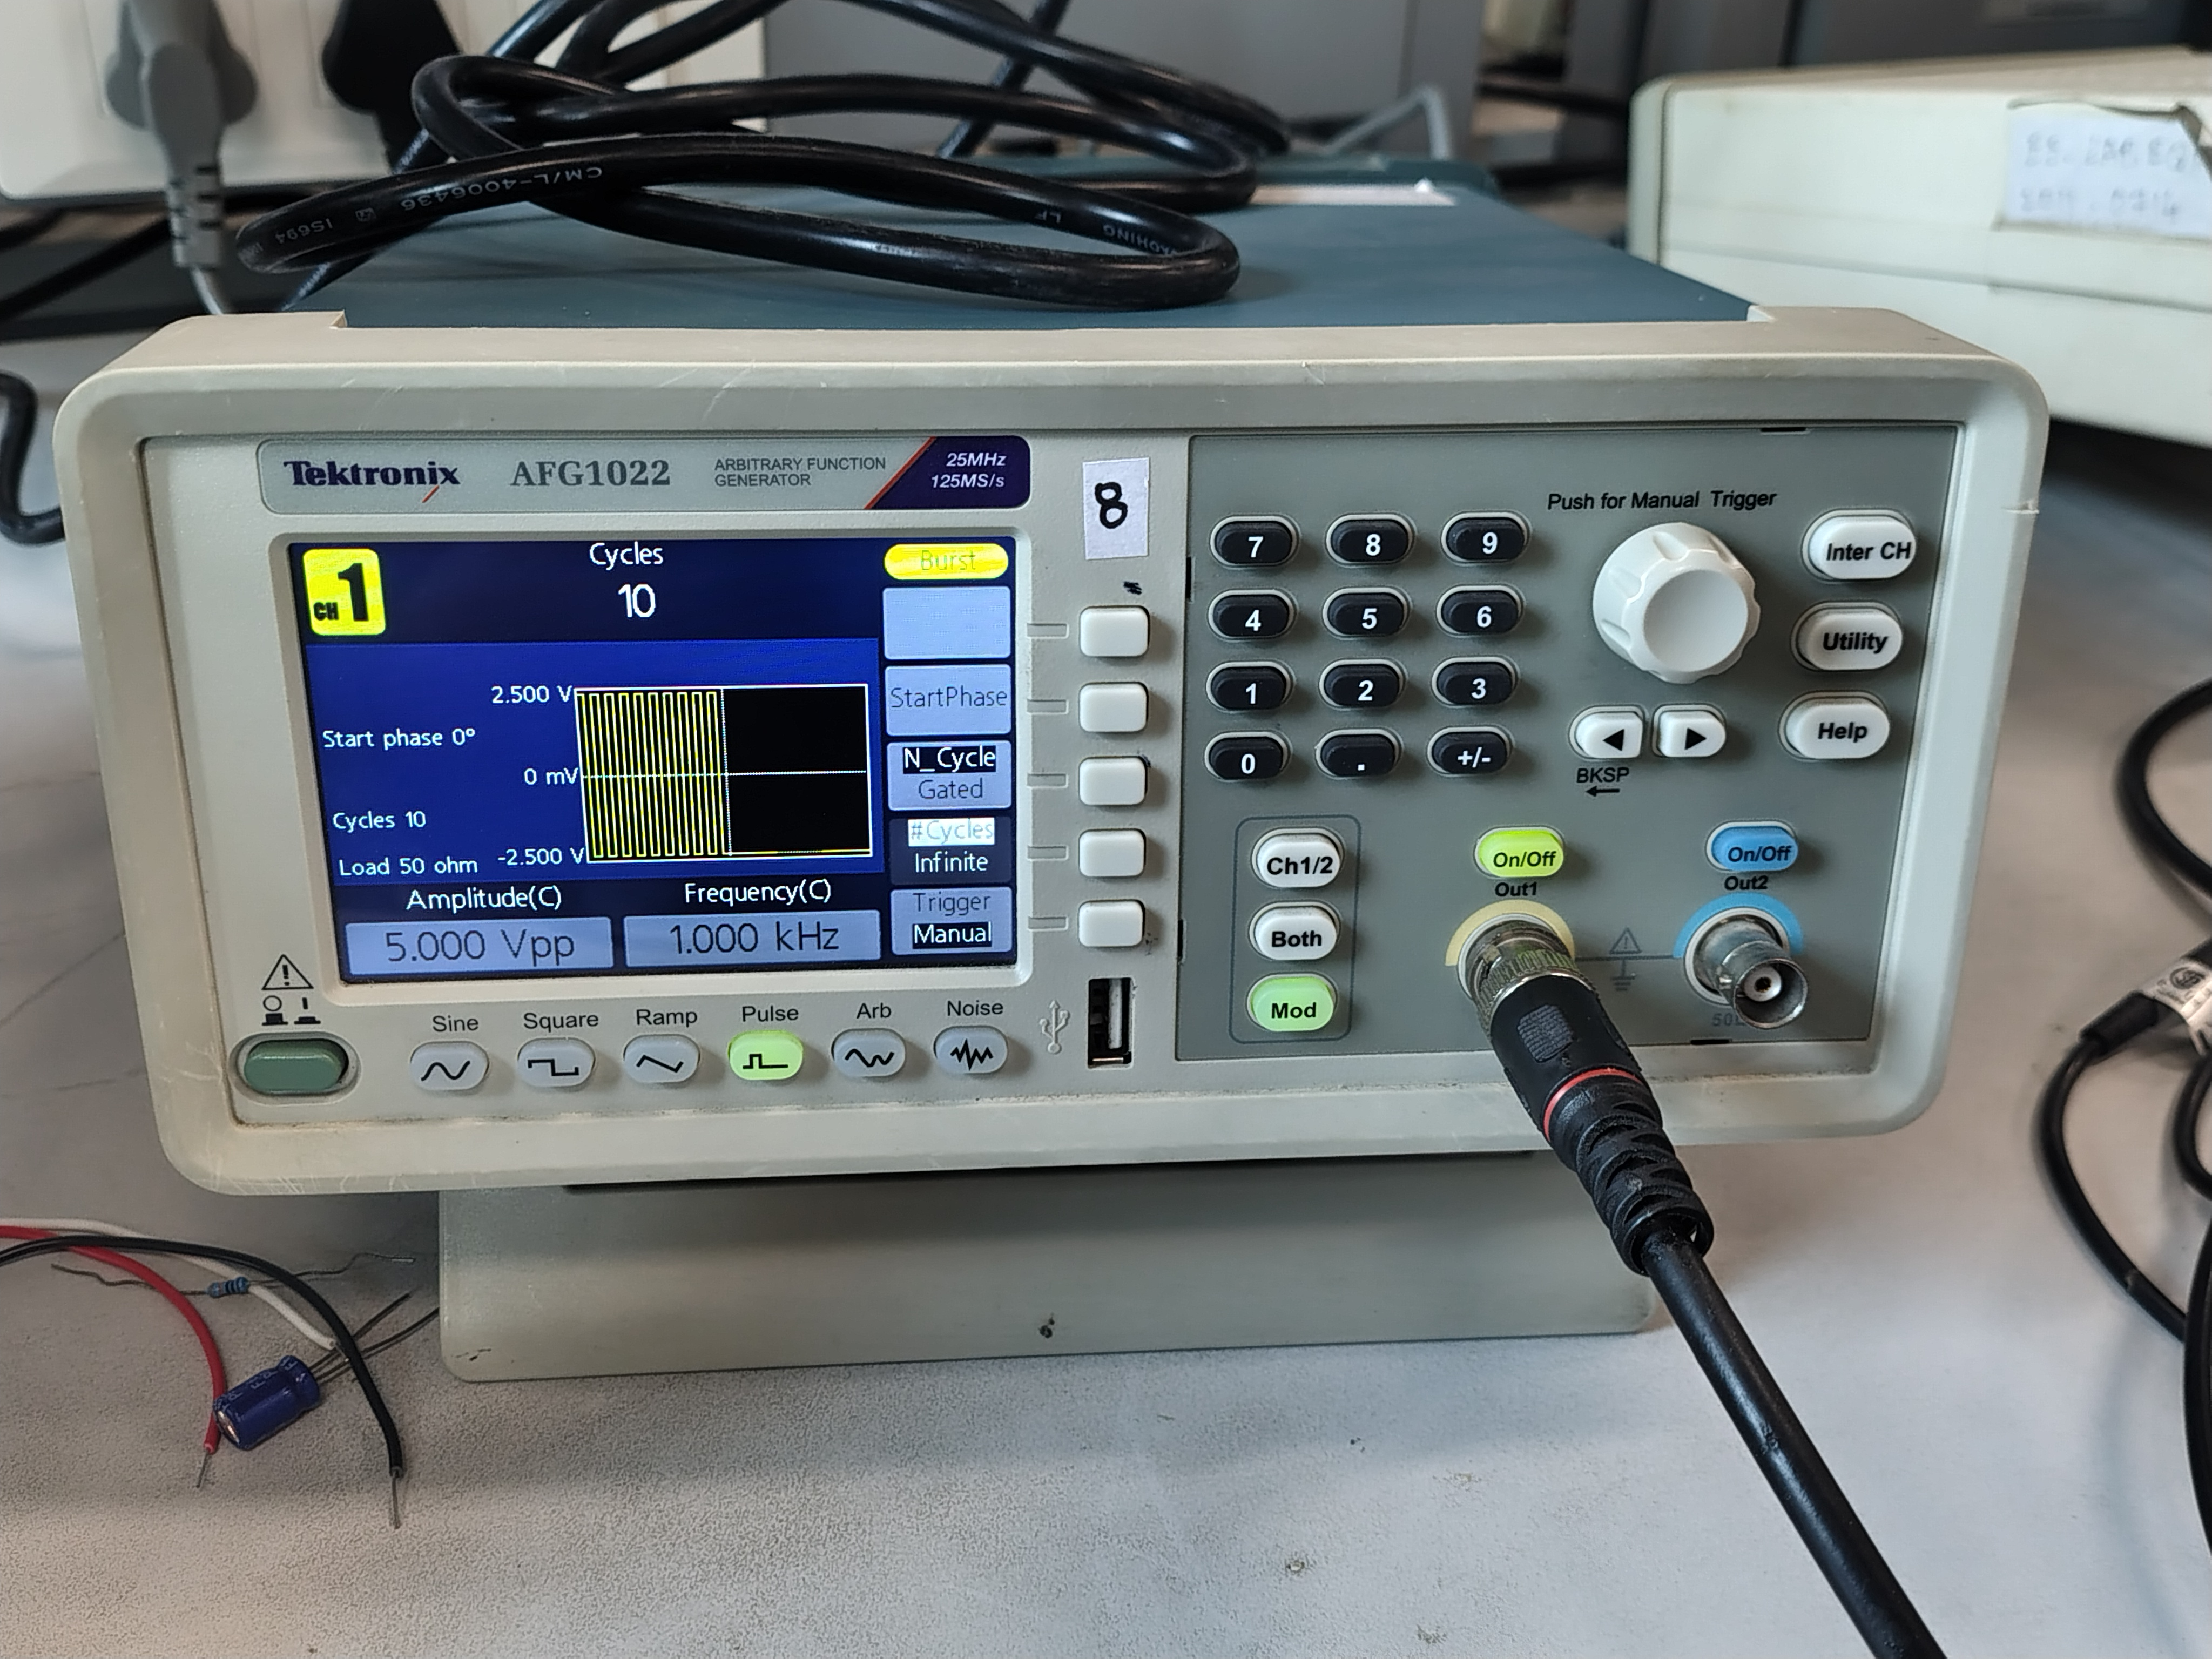
\includegraphics[width=0.7\textwidth]{figs/Experiment-2/1.2.2.jpg}
    \caption{Function generator configuration showing burst mode settings and manual trigger.}
    \label{fig:function_generator}
\end{figure}
\section{Conclusion}
This experiment successfully demonstrated the generation and analysis of Lissajous figures using a function generator and an oscilloscope, providing valuable insights into waveform behavior under varying frequency and phase conditions. Additionally, the methodology for capturing one-time events was effectively implemented, highlighting the importance of precise triggering and equipment configuration. These fundamental techniques are essential for signal analysis and troubleshooting in electrical engineering applications. The hands-on experience gained through this experiment enhances our practical understanding of waveform visualization, signal processing, and instrumentation, equipping us with critical skills for future experimental and professional endeavors.
\end{document}

